  % ============================================================
  %  CHAPTER 5: RELEASE 3 - ADVANCED SUPPORT AND INTELLIGENCE
  % ============================================================

  \fancyhead[L]{\fontsize{10}{12}\selectfont Chapter 5: Release 3 - Advanced Support and Intelligence}
  \fancyhead[R]{}
  \fancyfoot[C]{\thepage}
  \pagestyle{fancy}

  \phantomsection
  \addcontentsline{toc}{chapter}{Chapter 5: Release 3 - Advanced Support and Intelligence}

  \begin{center}
    {\fontsize{18}{22}\selectfont \textbf{Chapter 5}}
  \end{center}

  \vspace{0.3cm}

  \noindent\rule{\textwidth}{0.4pt}

  \vspace{0.3cm}

  \begin{center}
    {\fontsize{20}{24}\selectfont \textbf{Release 3 -- Advanced Support and Intelligence}}
  \end{center}

  \vspace{0.6cm}

  % ============================================================
  %  INTRODUCTION
  % ============================================================
  \ReportSection{Introduction}{Introduction}

  {\fontsize{12}{18}\selectfont
  \setlength{\parindent}{1.2cm}
  \setlength{\parskip}{6pt}

  \indent This chapter presents Release 3 of the ArabSoft platform. It covers the final advanced scope of the project through two sprints. Sprint 5 focuses on project management, task assignment, task progress tracking, and HR report export. Sprint 6 is reserved for AI assistance, deployment preparation, and final stabilization. Together, these elements complete the platform by adding collaboration, reporting, and intelligent support features on top of the workflows developed in the previous releases.

  }

  \vspace{6pt}

% ============================================================
%  I. RELEASE ORGANIZATION
% ============================================================
\ReportSection{I. Release Organization}{I. Release Organization}

{\fontsize{12}{18}\selectfont
\setlength{\parindent}{1.2cm}
\setlength{\parskip}{6pt}

\indent Release 3 is organized into two final sprints. Sprint 5 covers Projects, Tasks and Reports, while Sprint 6 covers AI, Deployment and Stabilization. This organization separates collaboration and reporting features from the assistant and stabilization work, making the final release easier to document and validate.

}

\begin{figure}[H]
  \centering
  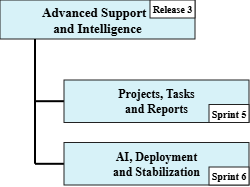
\includegraphics[width=0.62\textwidth,keepaspectratio]{sections/chapitre5/img/other/release3_organization.png}
  \caption{Release 3 Organization}
  \label{release3_organization}
\end{figure}

\vspace{6pt}

% ============================================================
%  II. SPRINT 5: PROJECTS, TASKS AND REPORTS
% ============================================================

\ReportSection{II. Sprint 5: Projects, Tasks and Reports}{II. Sprint 5: Projects, Tasks and Reports}

  \ReportSubsection{II.1 Sprint Goal}{\hspace{0.5cm} 1. Sprint Goal}

  {\fontsize{12}{18}\selectfont
  \setlength{\parindent}{1.2cm}
  \setlength{\parskip}{6pt}

  \indent This sprint focuses on project and task management for team leaders, assignee-side task progress tracking, and HR reporting through consultation and Excel export. It connects operational planning, task execution, and reporting features while keeping each workflow aligned with the implemented role permissions.

  }

  \ReportSubsection{II.2 Visual Sprint Journal}{\hspace{0.5cm} 2. Visual Sprint Journal}

  {\fontsize{12}{18}\selectfont
  \setlength{\parindent}{1.2cm}
  \setlength{\parskip}{6pt}

  \indent The visual sprint journal below presents the selected user stories of Sprint 5 and their completion status in Jira.

  }

  \begin{figure}[H]
    \centering
    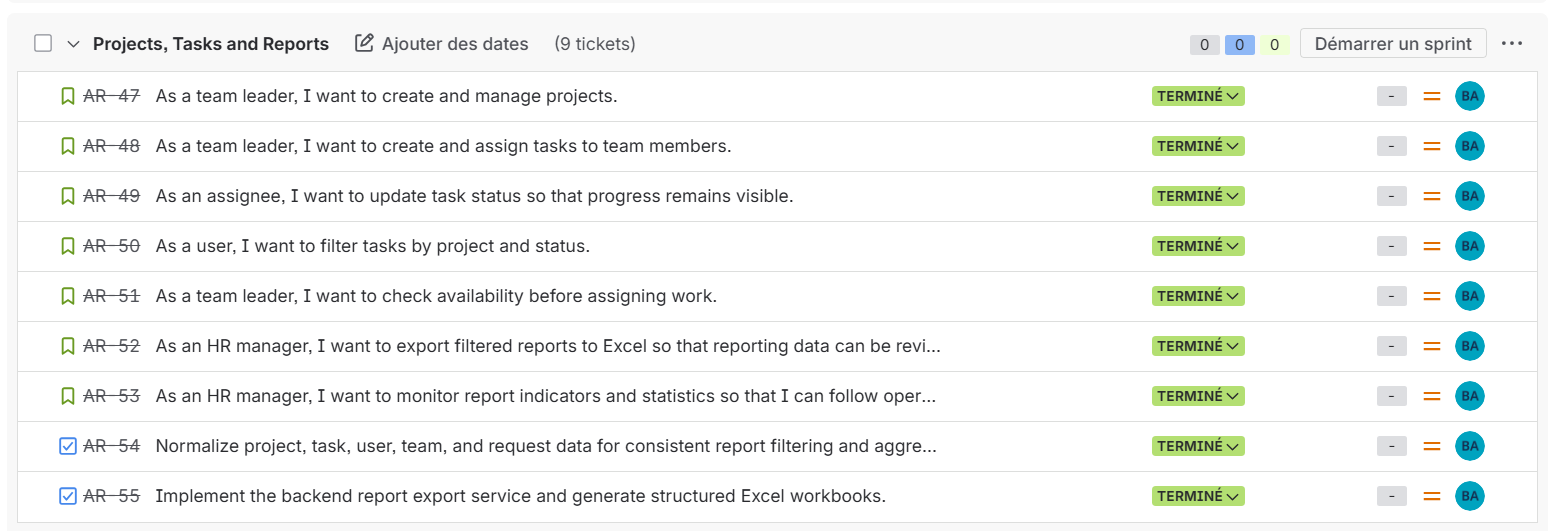
\includegraphics[width=0.95\textwidth,keepaspectratio]{sections/chapitre5/img/sprint5_projects_tasks_reports/01_jira/sprint5_jira_journal.png}
    \caption*{Visual Sprint Journal -- Sprint 5}
    \phantomsection\label{fig:sprint5_jira_journal}
  \end{figure}

  \ReportSubsection{II.3 Sprint Backlog}{\hspace{0.5cm} 3. Sprint Backlog}

  {\fontsize{12}{18}\selectfont
  \setlength{\parindent}{1.2cm}
  \setlength{\parskip}{6pt}

  \indent The table below summarizes the Sprint 5 work packages prepared from the product backlog defined in Chapter 2.

  }

  \begin{table}[H]
  \centering
  \normalsize
  \renewcommand{\arraystretch}{2.15}
  \setlength{\extrarowheight}{5pt}
  \setlength{\tabcolsep}{4pt}
  \begin{tabular}{|>{\centering\bfseries\arraybackslash}m{1.5cm}|>{\centering\bfseries\arraybackslash}m{3.6cm}|>{\RaggedRight\arraybackslash}m{7.4cm}|>{\centering\arraybackslash}m{1.6cm}|}
  \hline
  \rowcolor{blue!20}
  \textbf{Sprint} & \textbf{Stories} & \centering\textbf{Tasks} & \textbf{Duration} \\
  \hline
  \multirow{10}{=}{\centering\textbf{Sprint 5}}
  & \multirow{2}{=}{\centering\textbf{Project management}}
  & Create, update, delete, and view team-scoped projects
  & \multirow{2}{=}{\centering 2d} \\
  \cline{3-3}
  & & Keep project consultation limited to the connected team scope & \\
  \cline{2-4}
  & \multirow{3}{=}{\centering\textbf{Task creation and assignment}}
  & Create tasks and assign them using ONE, SELECTED, or ALL modes
  & \multirow{3}{=}{\centering 2d} \\
  \cline{3-3}
  & & Preview member availability before assigning tasks & \\
  \cline{3-3}
  & & Keep task assignment aligned with team membership and assignment mode rules & \\
  \cline{2-4}
  & \multirow{2}{=}{\centering\textbf{Task status update}}
  & Allow assigned users to update the task lifecycle from TODO to IN\_PROGRESS to DONE
  & \multirow{2}{=}{\centering 1d} \\
  \cline{3-3}
  & & Track assignee-side progress through the defined lifecycle states & \\
  \cline{2-4}
  & \multirow{3}{=}{\centering\textbf{HR reports consultation and Excel export}}
  & Consult leave, document, loan, and authorization report data
  & \multirow{3}{=}{\centering 2d} \\
  \cline{3-3}
  & & Filter report results before export & \\
  \cline{3-3}
  & & Export filtered HR reports to Excel & \\
  \hline
  \end{tabular}
  \caption*{Sprint Backlog -- Sprint 5}
  \phantomsection\label{tab:sprint5_backlog}
  \end{table}

  \clearpage
  \ReportSubsection{II.4 Sprint Implementation}{\hspace{0.5cm} 4. Sprint Implementation}

  {\fontsize{12}{18}\selectfont
  \setlength{\parindent}{1.2cm}
  \setlength{\parskip}{6pt}

  \indent The Sprint 5 implementation is presented through the following UML diagrams, covering project management, task assignment, task status update, and HR report export.

  }

  \vspace{6pt}

  \ReportSubsubsection{Requirements Analysis}

  {\fontsize{12}{18}\selectfont
  \setlength{\parindent}{1.2cm}
  \setlength{\parskip}{6pt}

  \indent The use case diagrams below show the main actor interactions for Sprint 5.

  }

  \Needspace{7.2cm}
  \begin{figure}[H]
    \centering
    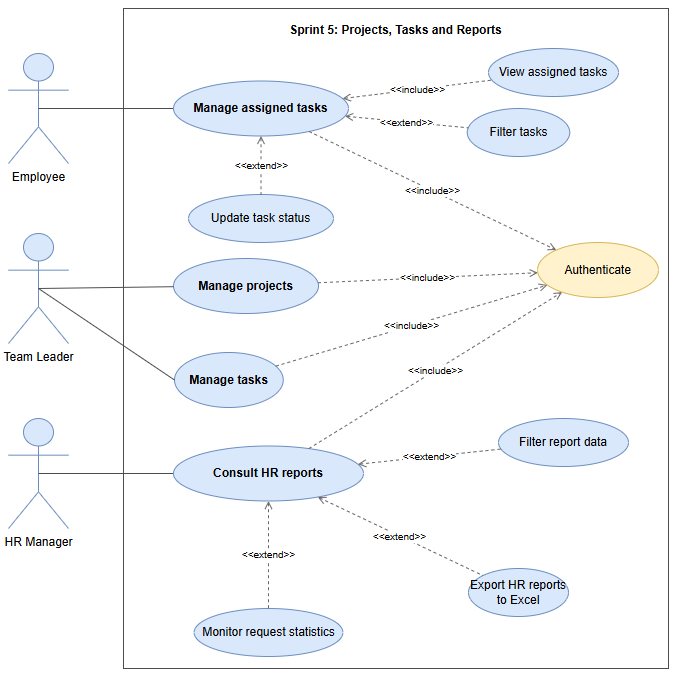
\includegraphics[width=0.95\textwidth,keepaspectratio]{sections/chapitre5/img/sprint5_projects_tasks_reports/02_use_case_diagrams/use_case_sprint5_projects_tasks_reports.png}
    \caption{Use Case Diagram – Sprint 5 Projects, Tasks and Reports}
    \label{fig:sprint5_projects_tasks_reports_use_case}
  \end{figure}

  \Needspace{7.2cm}
  \begin{figure}[H]
    \centering
    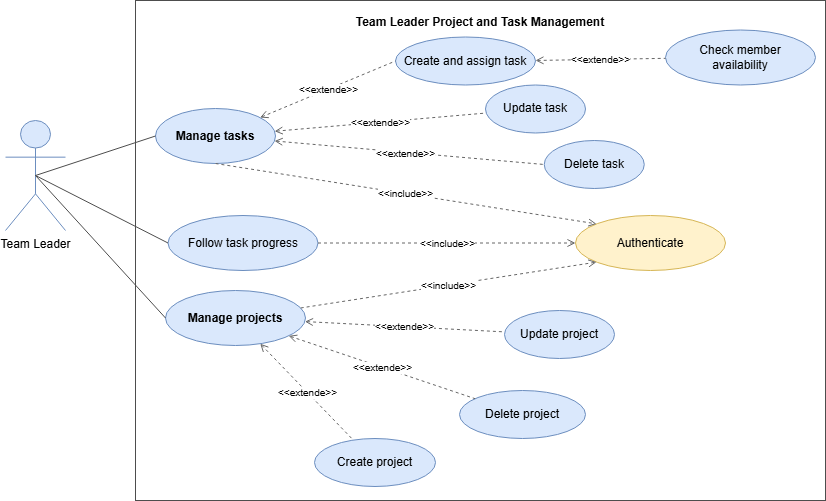
\includegraphics[width=0.95\textwidth,keepaspectratio]{sections/chapitre5/img/sprint5_projects_tasks_reports/02_use_case_diagrams/use_case_team_leader_project_task_management.png}
    \caption{Use Case Diagram – Team Leader Project and Task Management}
    \label{fig:team_leader_project_task_management_use_case}
  \end{figure}

  \vspace{6pt}

  \ReportSubsubsection{System Sequence Diagrams}

  {\fontsize{12}{18}\selectfont
  \setlength{\parindent}{1.2cm}
  \setlength{\parskip}{6pt}

  \indent These diagrams show how the user and system interact for the main Sprint 5 operations.

  }

  \Needspace{7.2cm}
  \begin{figure}[H]
    \centering
    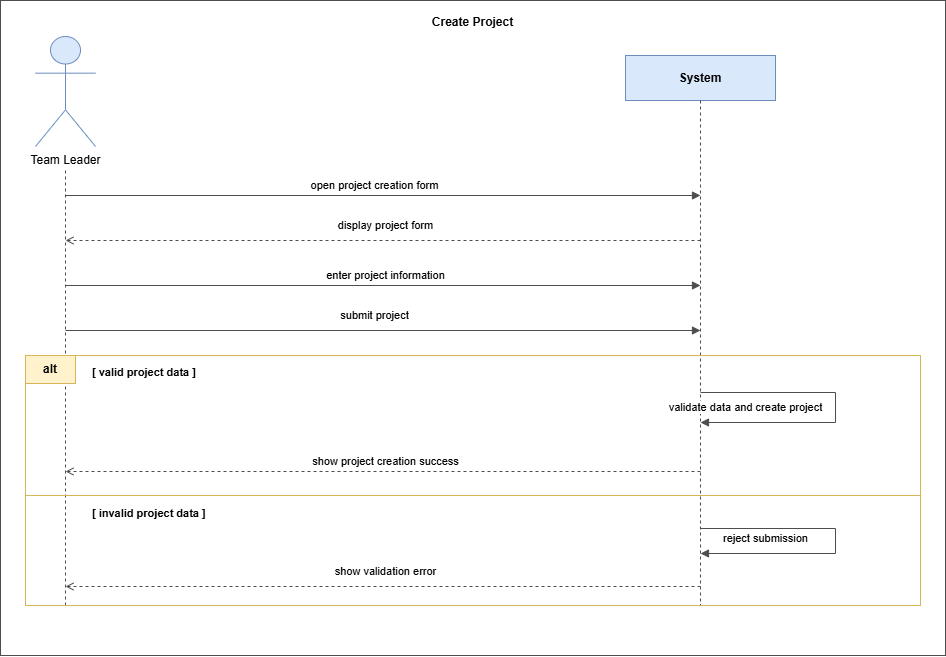
\includegraphics[width=0.95\textwidth,keepaspectratio]{sections/chapitre5/img/sprint5_projects_tasks_reports/03_system_sequence_diagrams/ssd_create_project.png}
    \caption{System Sequence Diagram – Create Project}
    \label{fig:ssd_create_project}
  \end{figure}

  \Needspace{7.2cm}
  \begin{figure}[H]
    \centering
    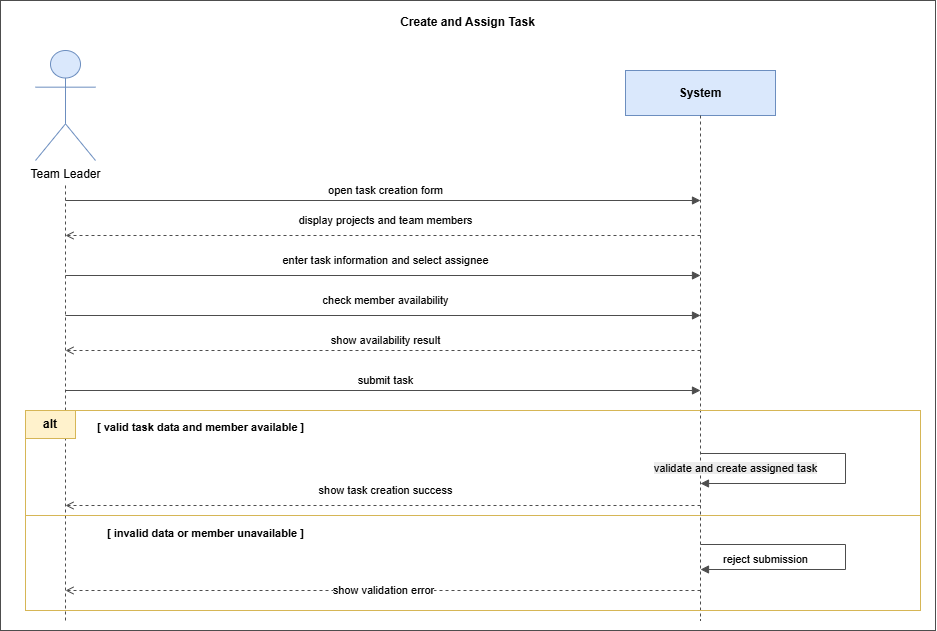
\includegraphics[width=0.95\textwidth,keepaspectratio]{sections/chapitre5/img/sprint5_projects_tasks_reports/03_system_sequence_diagrams/ssd_create_and_assign_task.png}
    \caption{System Sequence Diagram – Create and Assign Task}
    \label{fig:ssd_create_and_assign_task}
  \end{figure}

  \Needspace{7.2cm}
  \begin{figure}[H]
    \centering
    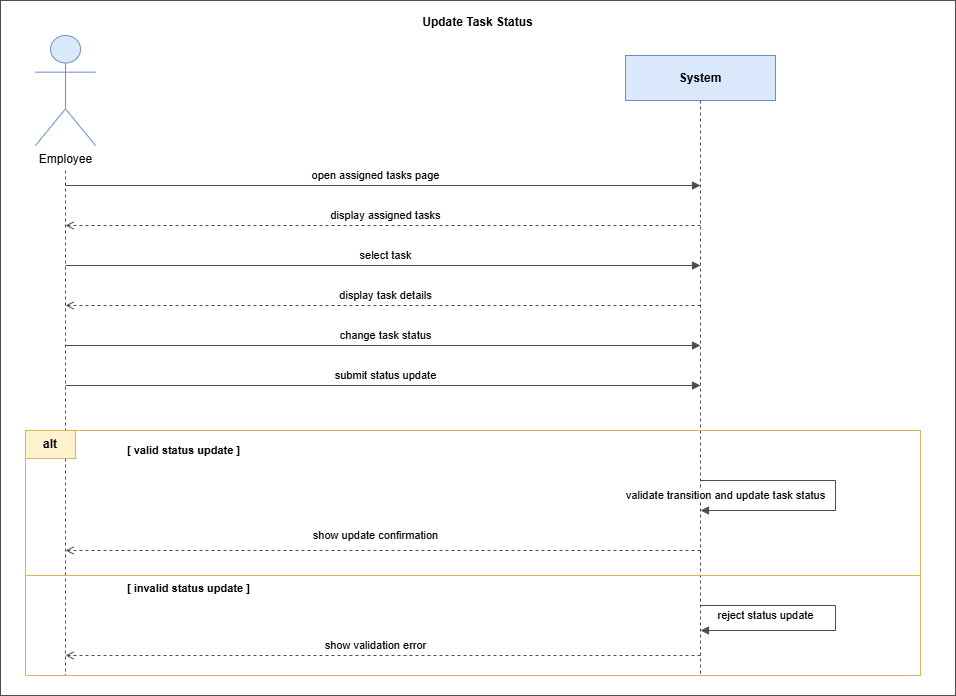
\includegraphics[width=0.95\textwidth,keepaspectratio]{sections/chapitre5/img/sprint5_projects_tasks_reports/03_system_sequence_diagrams/ssd_update_task_status.png}
    \caption{System Sequence Diagram – Update Task Status}
    \label{fig:ssd_update_task_status}
  \end{figure}

  \Needspace{7.2cm}
  \begin{figure}[H]
    \centering
    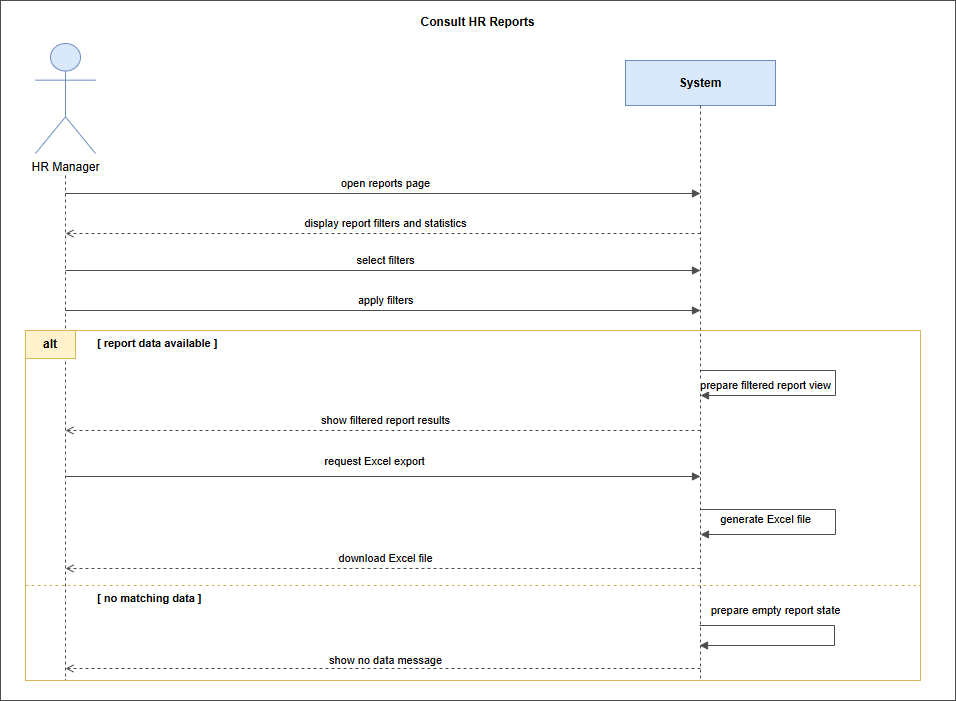
\includegraphics[width=0.95\textwidth,keepaspectratio]{sections/chapitre5/img/sprint5_projects_tasks_reports/03_system_sequence_diagrams/ssd_consult_hr_reports.png}
    \caption{System Sequence Diagram – Consult HR Reports}
    \label{fig:ssd_consult_hr_reports}
  \end{figure}

  \vspace{6pt}

  \ReportSubsubsection{Analysis}

  {\fontsize{12}{18}\selectfont
  \setlength{\parindent}{1.2cm}
  \setlength{\parskip}{6pt}

  \indent This diagram shows the main domain concepts behind Sprint 5's project management, task assignment, and reporting features.

  }

  \Needspace{7.2cm}
  \ChapterFourFigureSized
  {sections/chapitre5/img/sprint5_projects_tasks_reports/05_domain_model/domain_model_sprint5_projects_tasks_reports.png}
  {Domain Model -- Sprint 5 Projects, Tasks and Reports}
  {domain_model_sprint5_projects_tasks_reports}
  {0.95}

  \vspace{6pt}

  \ReportSubsubsection{State Diagrams}

  {\fontsize{11}{14}\selectfont
  \setlength{\parindent}{1.2cm}
  \setlength{\parskip}{2pt}

  \indent The state diagram below shows the task lifecycle for Sprint 5: TODO, IN\_PROGRESS, and DONE.

  }

  \vspace{-6pt}

  \begin{figure}[H]
    \centering
    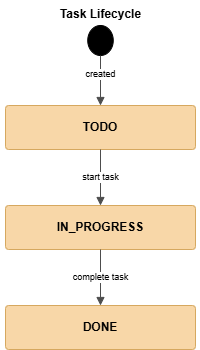
\includegraphics[height=6.8cm,keepaspectratio]{sections/chapitre5/img/sprint5_projects_tasks_reports/04_state_diagrams/state_task_lifecycle.png}
    \caption{State Diagram -- Task Lifecycle}
    \label{fig:state_task_lifecycle}
  \end{figure}

  \vspace{-4pt}
  \Needspace{10cm}

  \ReportSubsubsection{Participant Class Diagrams}

  {\fontsize{12}{18}\selectfont
  \setlength{\parindent}{1.2cm}
  \setlength{\parskip}{6pt}

  \indent The participant class diagrams below show the frontend and backend classes involved in the main Sprint 5 workflows.

  }

  \Needspace{7.2cm}
  \begin{figure}[H]
    \centering
    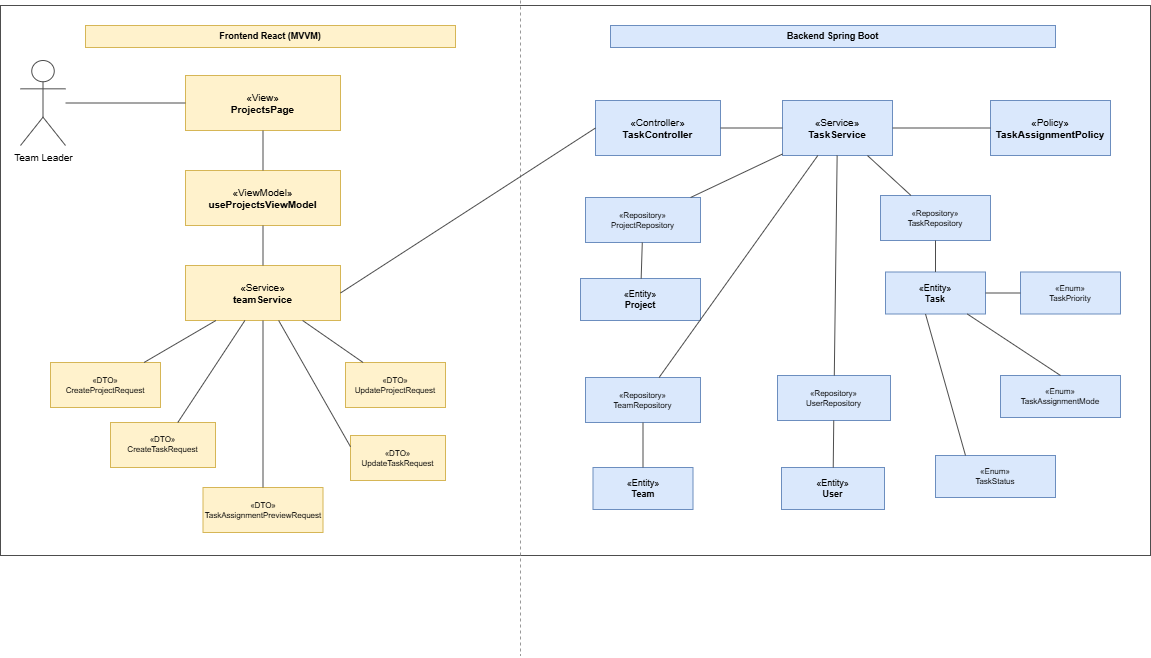
\includegraphics[width=0.95\textwidth,keepaspectratio]{sections/chapitre5/img/sprint5_projects_tasks_reports/06_participant_class_diagrams/participant_team_leader_project_management.png}
    \caption{Participant Class Diagram -- Team Leader Project and Task Management}
    \label{fig:participant_team_leader_project_management}
  \end{figure}

  \Needspace{7.2cm}
  \begin{figure}[H]
    \centering
    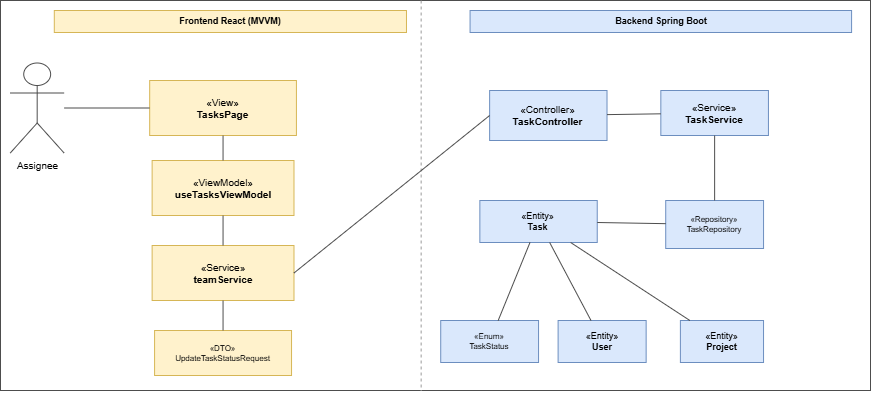
\includegraphics[width=0.95\textwidth,keepaspectratio]{sections/chapitre5/img/sprint5_projects_tasks_reports/06_participant_class_diagrams/participant_task_status_update.png}
    \caption{Participant Class Diagram -- Task Status Update}
    \label{fig:participant_task_status_update}
  \end{figure}

  \Needspace{7.2cm}
  \begin{figure}[H]
    \centering
    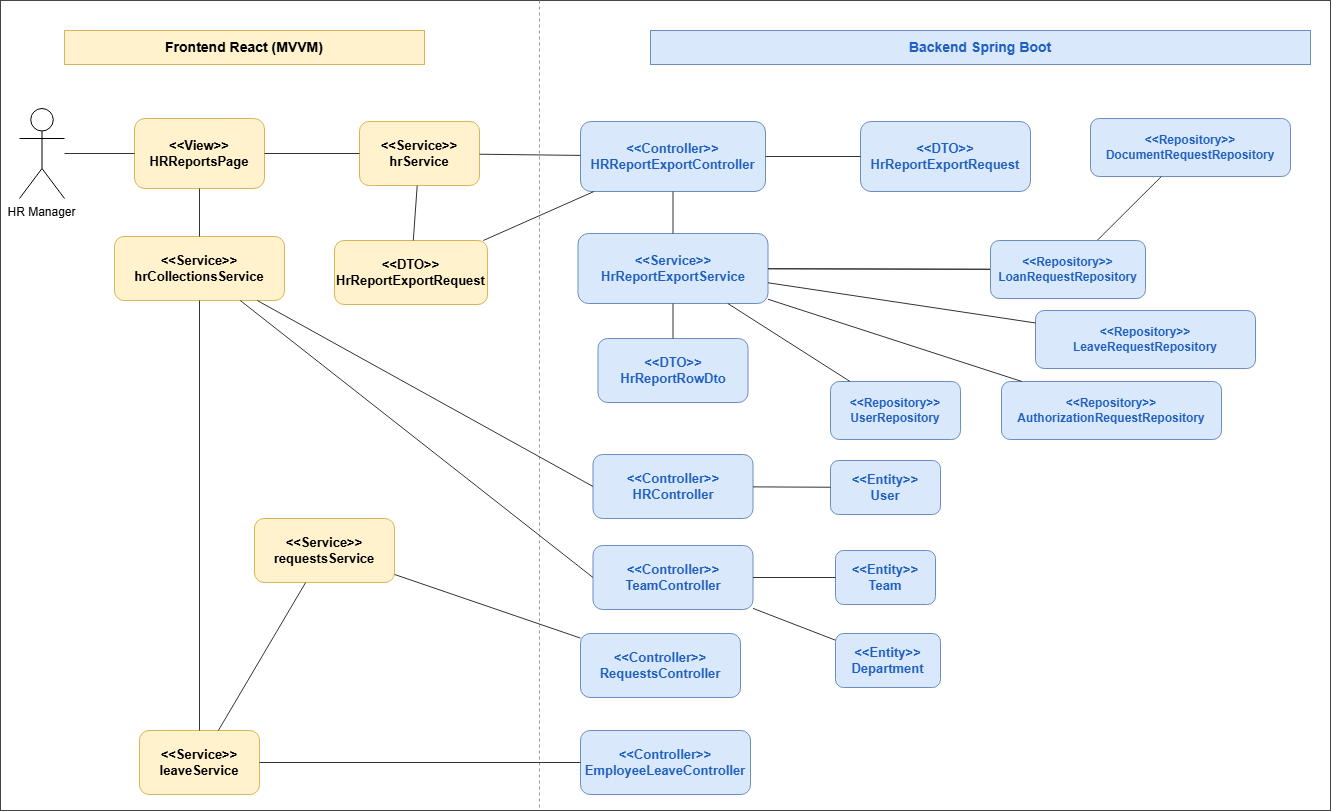
\includegraphics[width=0.95\textwidth,keepaspectratio]{sections/chapitre5/img/sprint5_projects_tasks_reports/06_participant_class_diagrams/participant_hr_reports_export.png}
    \caption{Participant Class Diagram -- HR Reports and Export}
    \label{fig:participant_hr_reports_export}
  \end{figure}

  \vspace{6pt}

  \ReportSubsubsection{Design Class Diagrams}

  {\fontsize{12}{18}\selectfont
  \setlength{\parindent}{1.2cm}
  \setlength{\parskip}{6pt}

  \indent The design class diagrams below show the class structure for Sprint 5 project management, task handling, and HR report export.

  }

  \Needspace{7.2cm}
  \begin{figure}[H]
    \centering
    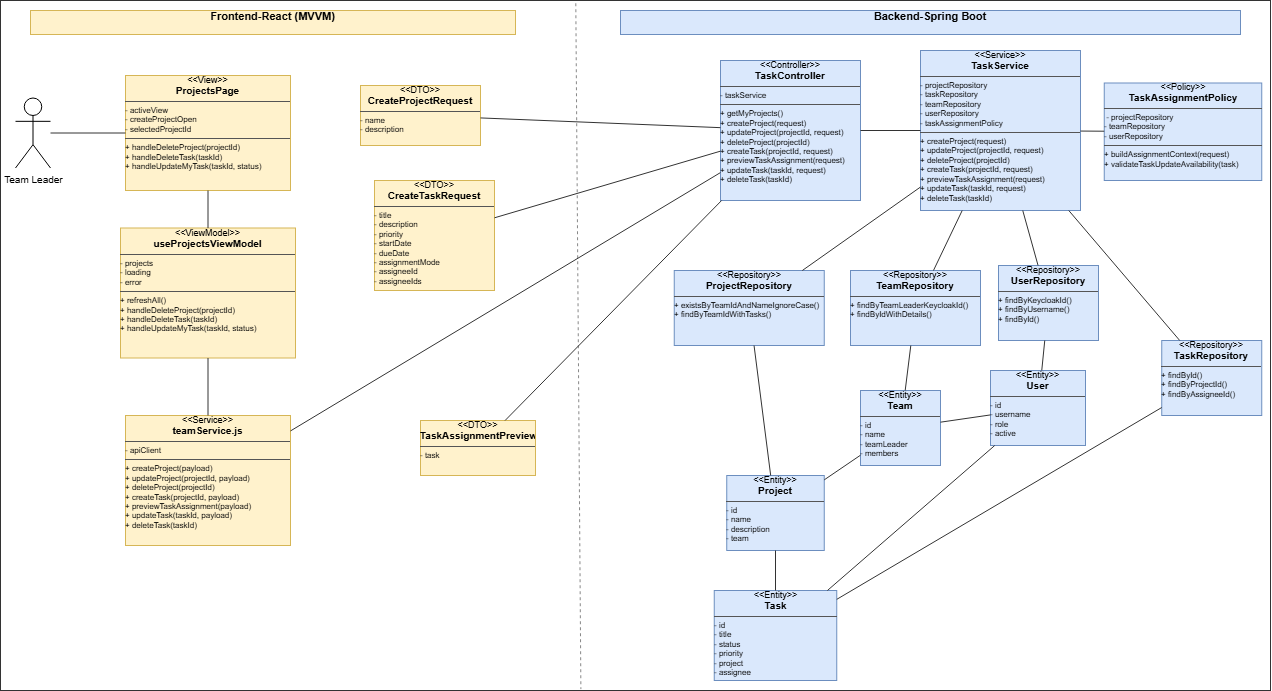
\includegraphics[width=0.95\textwidth,keepaspectratio]{sections/chapitre5/img/sprint5_projects_tasks_reports/07_design_class_diagrams/design_class_diagram_team_leader_project_task_management.png}
    \caption{Design Class Diagram -- Team Leader Project and Task Management}
    \label{fig:design_class_diagram_team_leader_project_task_management}
  \end{figure}

  \Needspace{7.2cm}
  \begin{figure}[H]
    \centering
    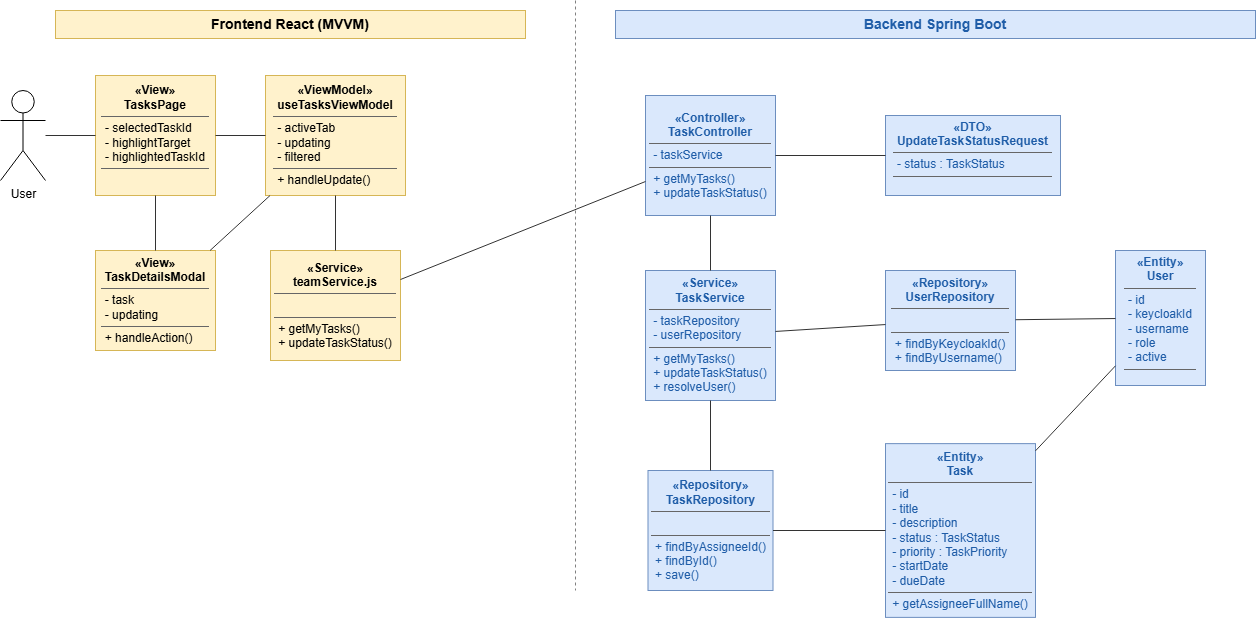
\includegraphics[width=0.95\textwidth,keepaspectratio]{sections/chapitre5/img/sprint5_projects_tasks_reports/07_design_class_diagrams/design_class_diagram_task_status_update.png}
    \caption{Design Class Diagram -- Task Status Update}
    \label{fig:design_class_diagram_task_status_update}
  \end{figure}

  \Needspace{7.2cm}
  \begin{figure}[H]
    \centering
    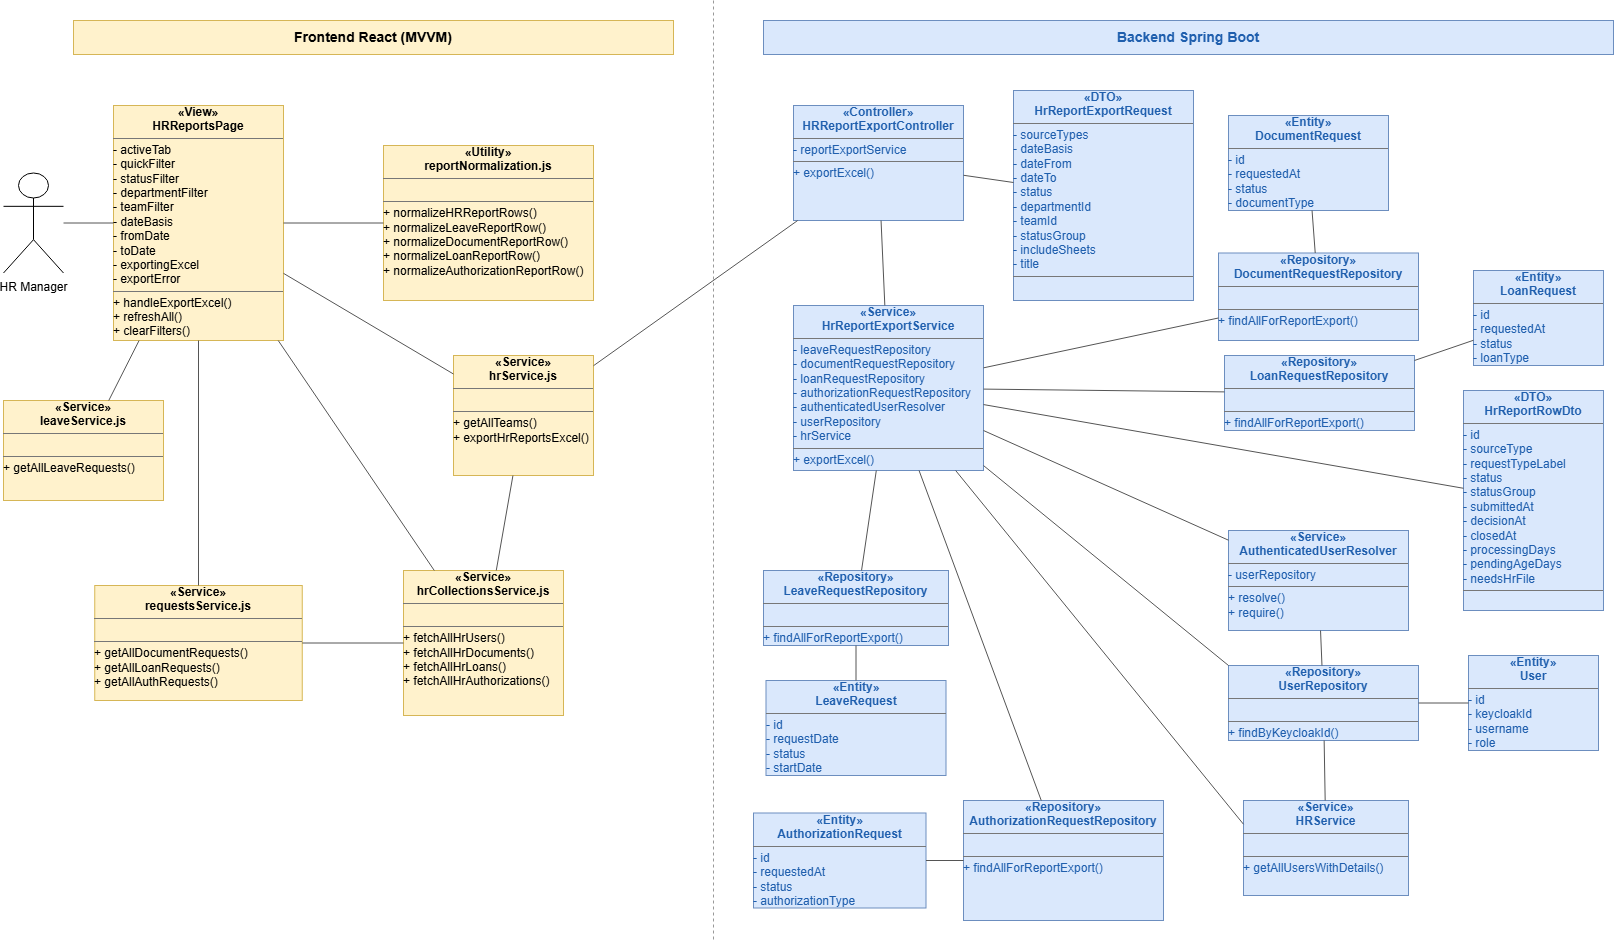
\includegraphics[width=0.95\textwidth,keepaspectratio]{sections/chapitre5/img/sprint5_projects_tasks_reports/07_design_class_diagrams/design_class_diagram_hr_reports_excel_export.png}
    \caption{Design Class Diagram -- HR Reports and Excel Export}
    \label{fig:design_class_diagram_hr_reports_excel_export}
  \end{figure}

  \vspace{6pt}

  \ReportSubsubsection{Conception Sequence Diagrams}

  {\fontsize{12}{18}\selectfont
  \setlength{\parindent}{1.2cm}
  \setlength{\parskip}{6pt}

  \indent The conception sequence diagrams below show the frontend and backend interactions for project management, task assignment, and status update.

  }

  \Needspace{7.2cm}
  \begin{figure}[H]
    \centering
    \makebox[\textwidth][c]{%
      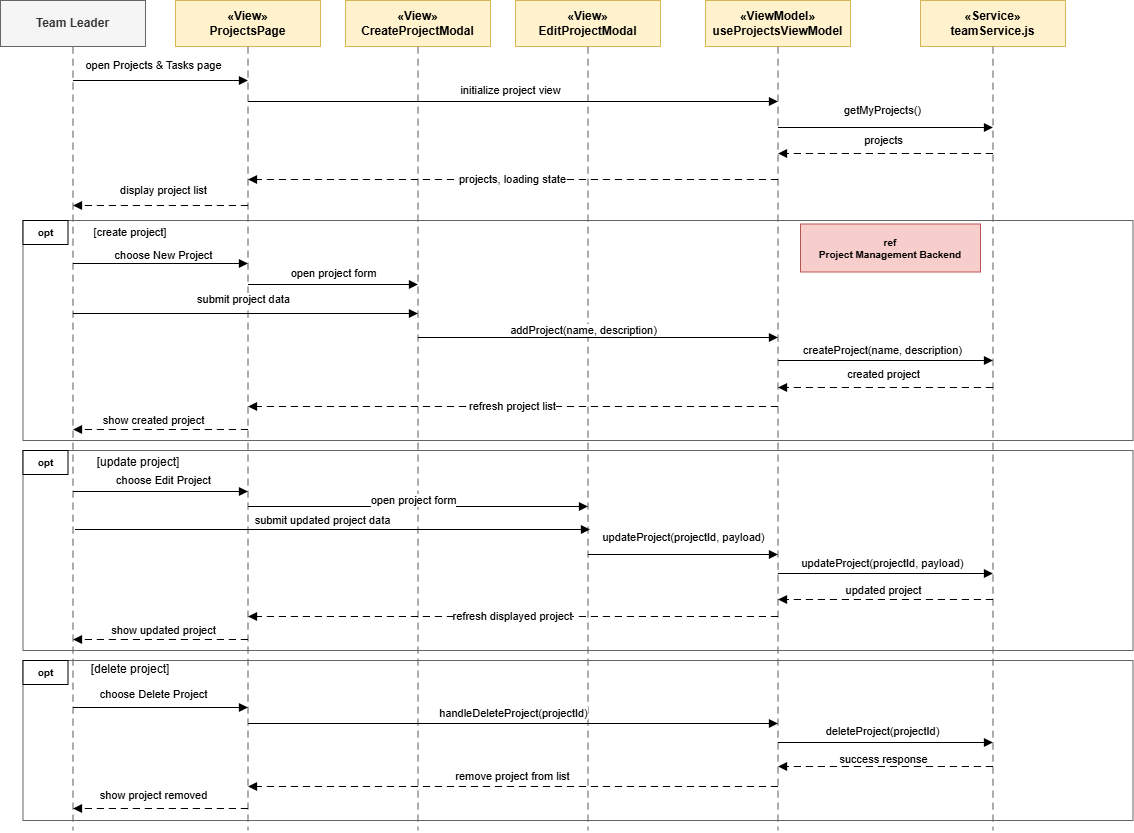
\includegraphics[width=1.10\textwidth,height=0.76\textheight]{sections/chapitre5/img/sprint5_projects_tasks_reports/08_conception_sequence_diagrams/csd_project_management_frontend.png}%
    }
    \caption{Conception Sequence Diagram -- Project Management Frontend}
    \label{fig:csd_project_management_frontend}
  \end{figure}

  \Needspace{7.2cm}
  \begin{figure}[H]
    \centering
    \makebox[\textwidth][c]{%
      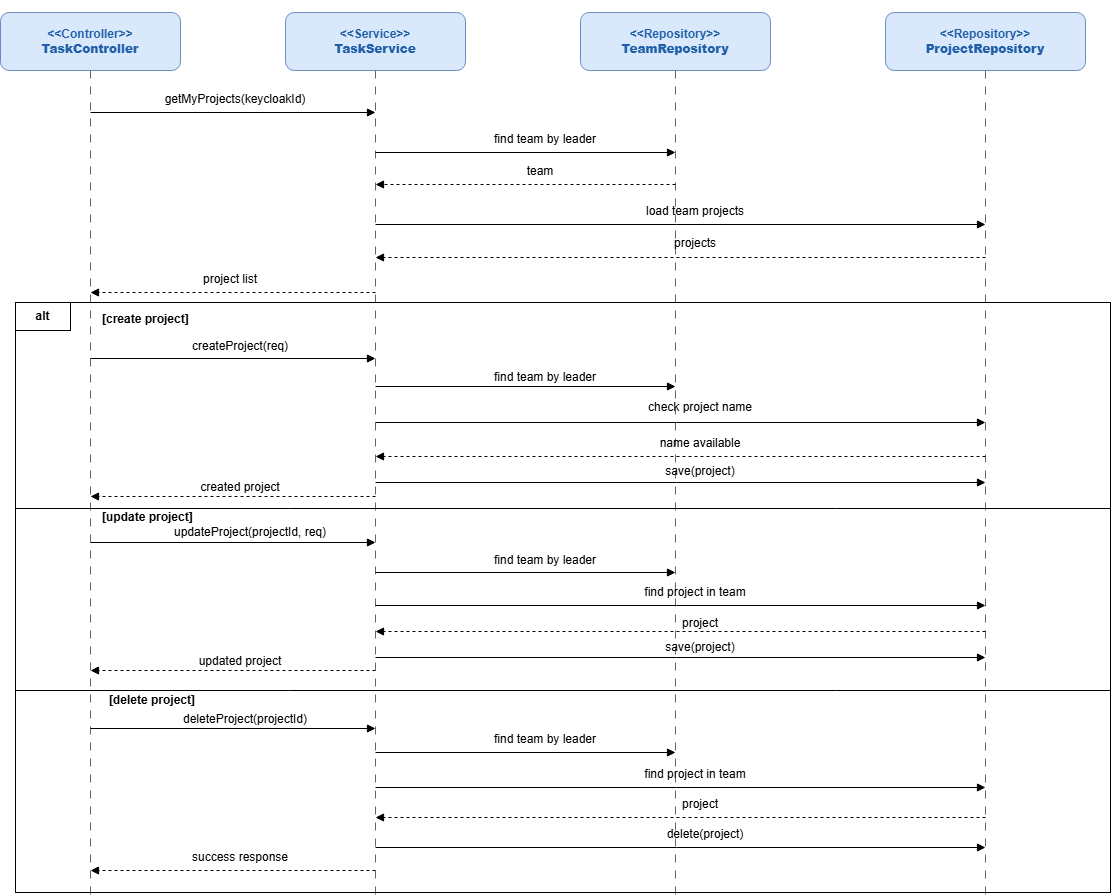
\includegraphics[width=1.10\textwidth,height=0.76\textheight]{sections/chapitre5/img/sprint5_projects_tasks_reports/08_conception_sequence_diagrams/csd_project_management_backend.png}%
    }
    \caption{Conception Sequence Diagram -- Project Management Backend}
    \label{fig:csd_project_management_backend}
  \end{figure}

  \Needspace{7.2cm}
  \begin{figure}[H]
    \centering
    \makebox[\textwidth][c]{%
      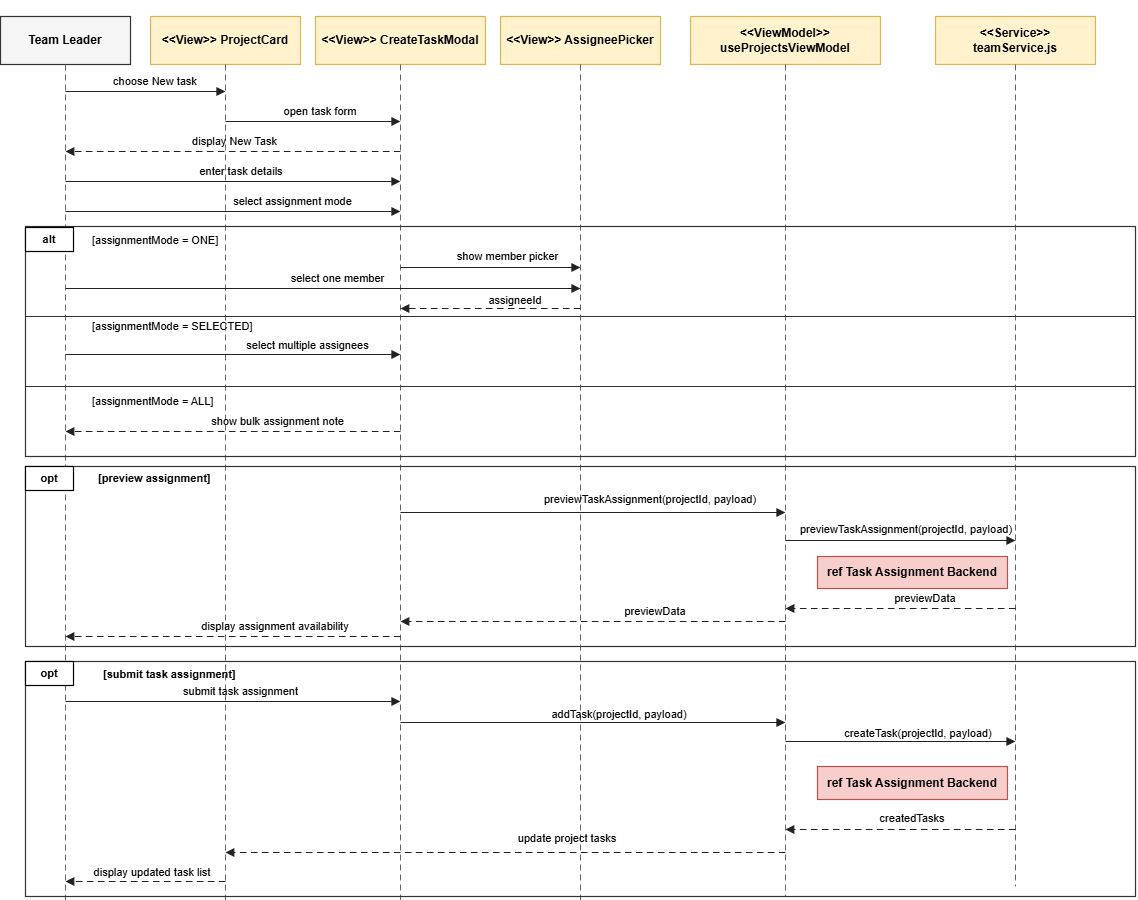
\includegraphics[width=1.10\textwidth,height=0.76\textheight]{sections/chapitre5/img/sprint5_projects_tasks_reports/08_conception_sequence_diagrams/csd_task_assignment_frontend.png}%
    }
    \caption{Conception Sequence Diagram -- Task Assignment Frontend}
    \label{fig:csd_task_assignment_frontend}
  \end{figure}

  \Needspace{7.2cm}
  \begin{figure}[H]
    \centering
    \makebox[\textwidth][c]{%
      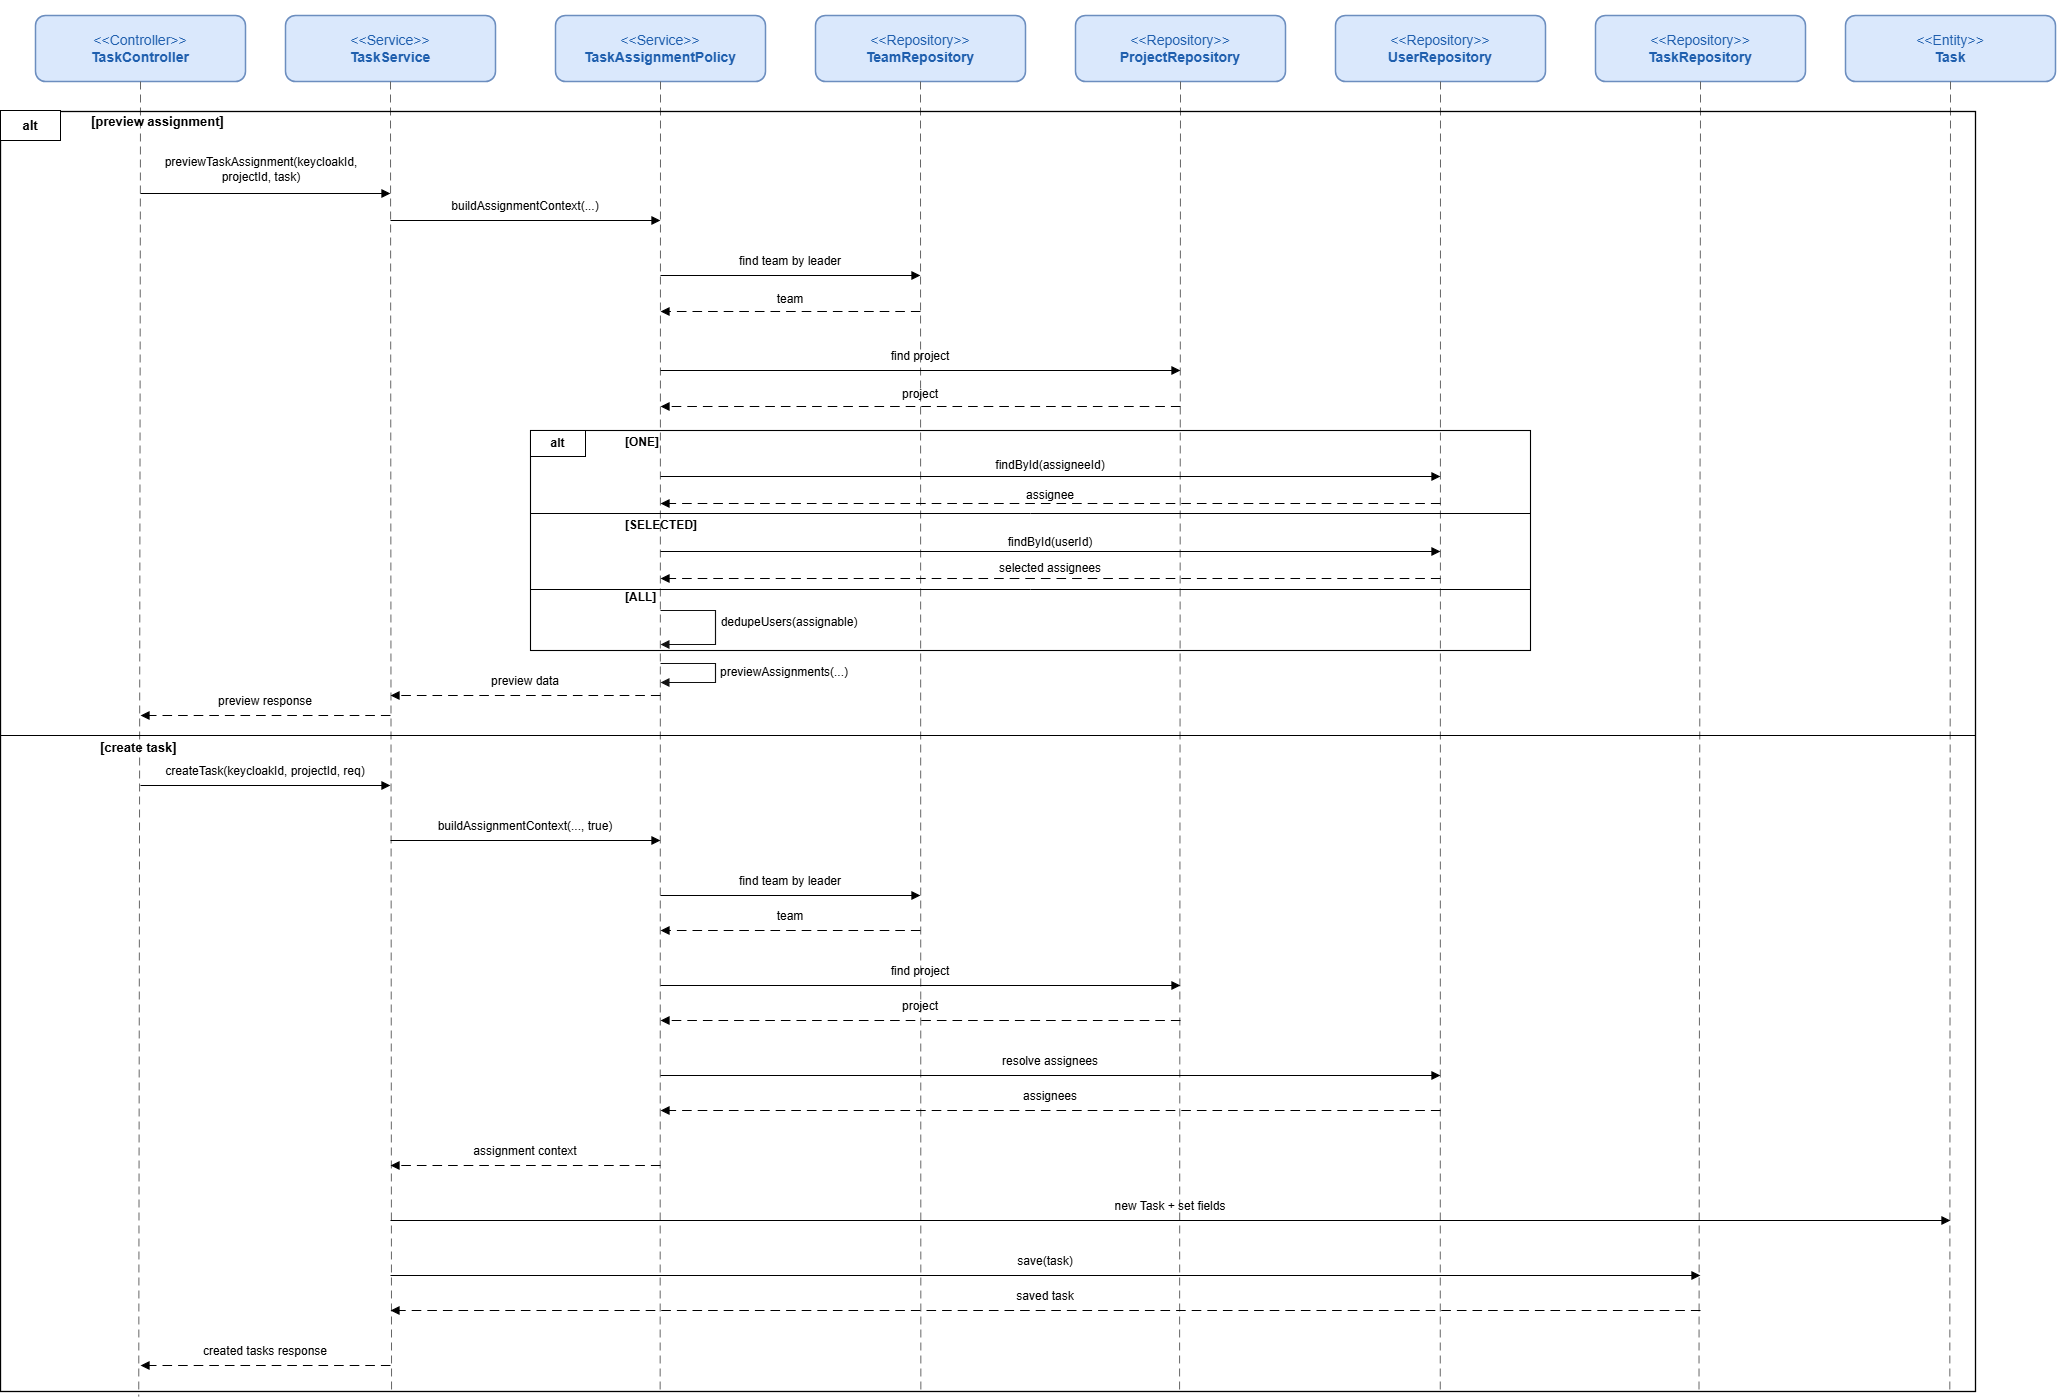
\includegraphics[width=1.10\textwidth,height=0.76\textheight]{sections/chapitre5/img/sprint5_projects_tasks_reports/08_conception_sequence_diagrams/csd_task_assignment_backend.png}%
    }
    \caption{Conception Sequence Diagram -- Task Assignment Backend}
    \label{fig:csd_task_assignment_backend}
  \end{figure}

  \Needspace{7.2cm}
  \begin{figure}[H]
    \centering
    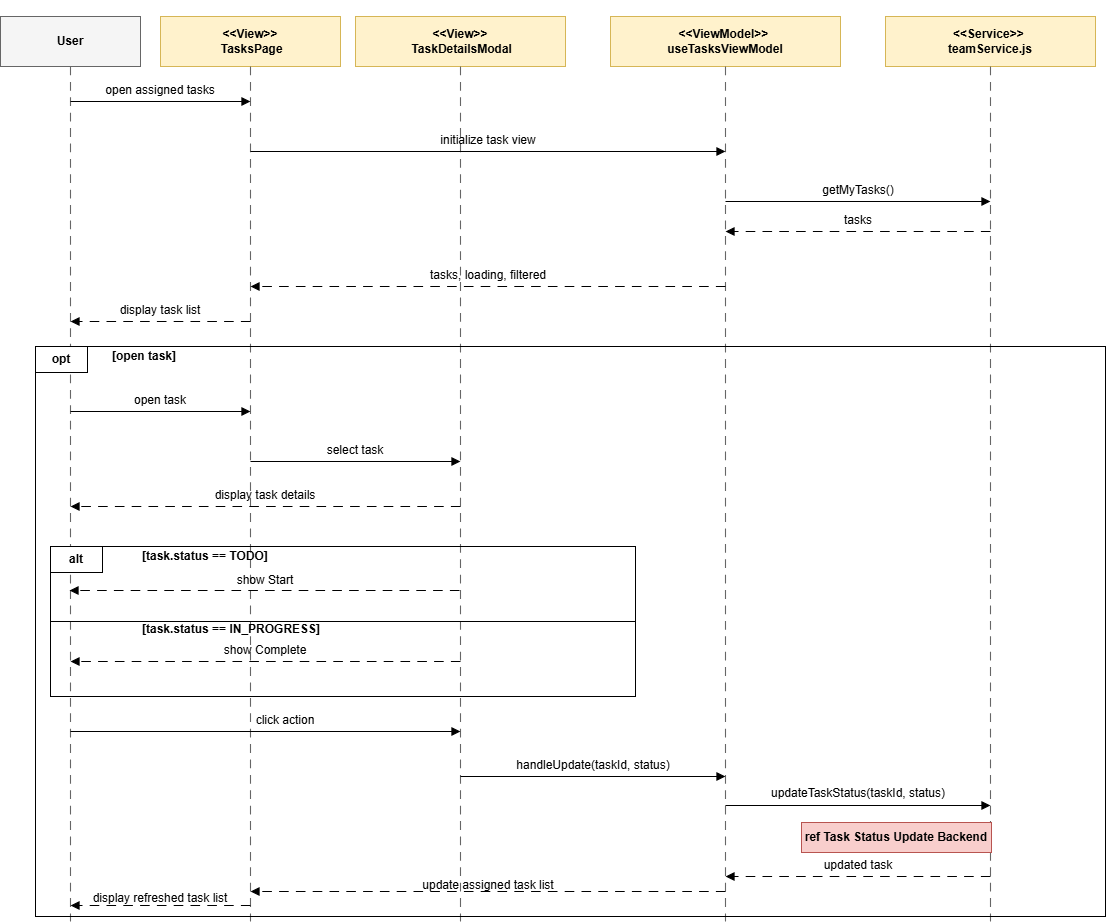
\includegraphics[width=0.95\textwidth,height=0.82\textheight,keepaspectratio]{sections/chapitre5/img/sprint5_projects_tasks_reports/08_conception_sequence_diagrams/csd_task_status_update_frontend.png}
    \caption{Conception Sequence Diagram -- Task Status Update Frontend}
    \label{fig:csd_task_status_update_frontend}
  \end{figure}

  \Needspace{7.2cm}
  \begin{figure}[H]
    \centering
    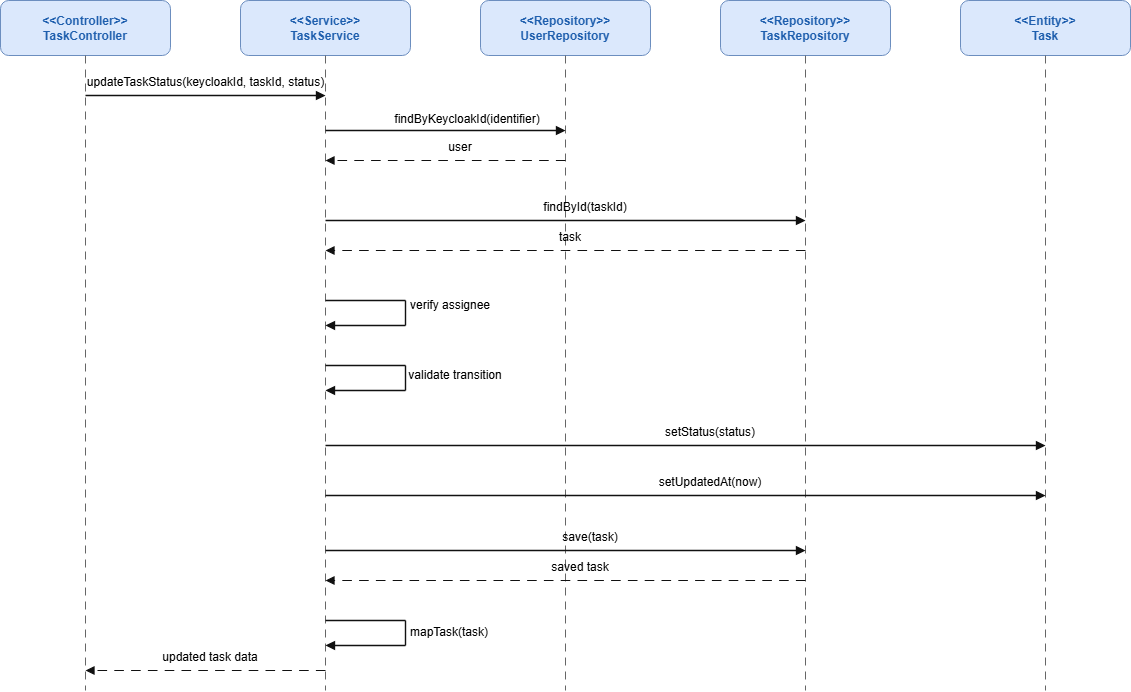
\includegraphics[width=0.95\textwidth,height=0.82\textheight,keepaspectratio]{sections/chapitre5/img/sprint5_projects_tasks_reports/08_conception_sequence_diagrams/csd_task_status_update_backend.png}
    \caption{Conception Sequence Diagram -- Task Status Update Backend}
    \label{fig:csd_task_status_update_backend}
  \end{figure}

  \ReportSubsubsection{Interface Screenshots}

  {\fontsize{12}{18}\selectfont
  \setlength{\parindent}{1.2cm}
  \setlength{\parskip}{6pt}

  \indent The following screenshots document the Sprint 5 user interfaces for projects, tasks, reporting, and Excel export.

  }

  \Needspace{7.2cm}
  \begin{figure}[H]
    \centering
    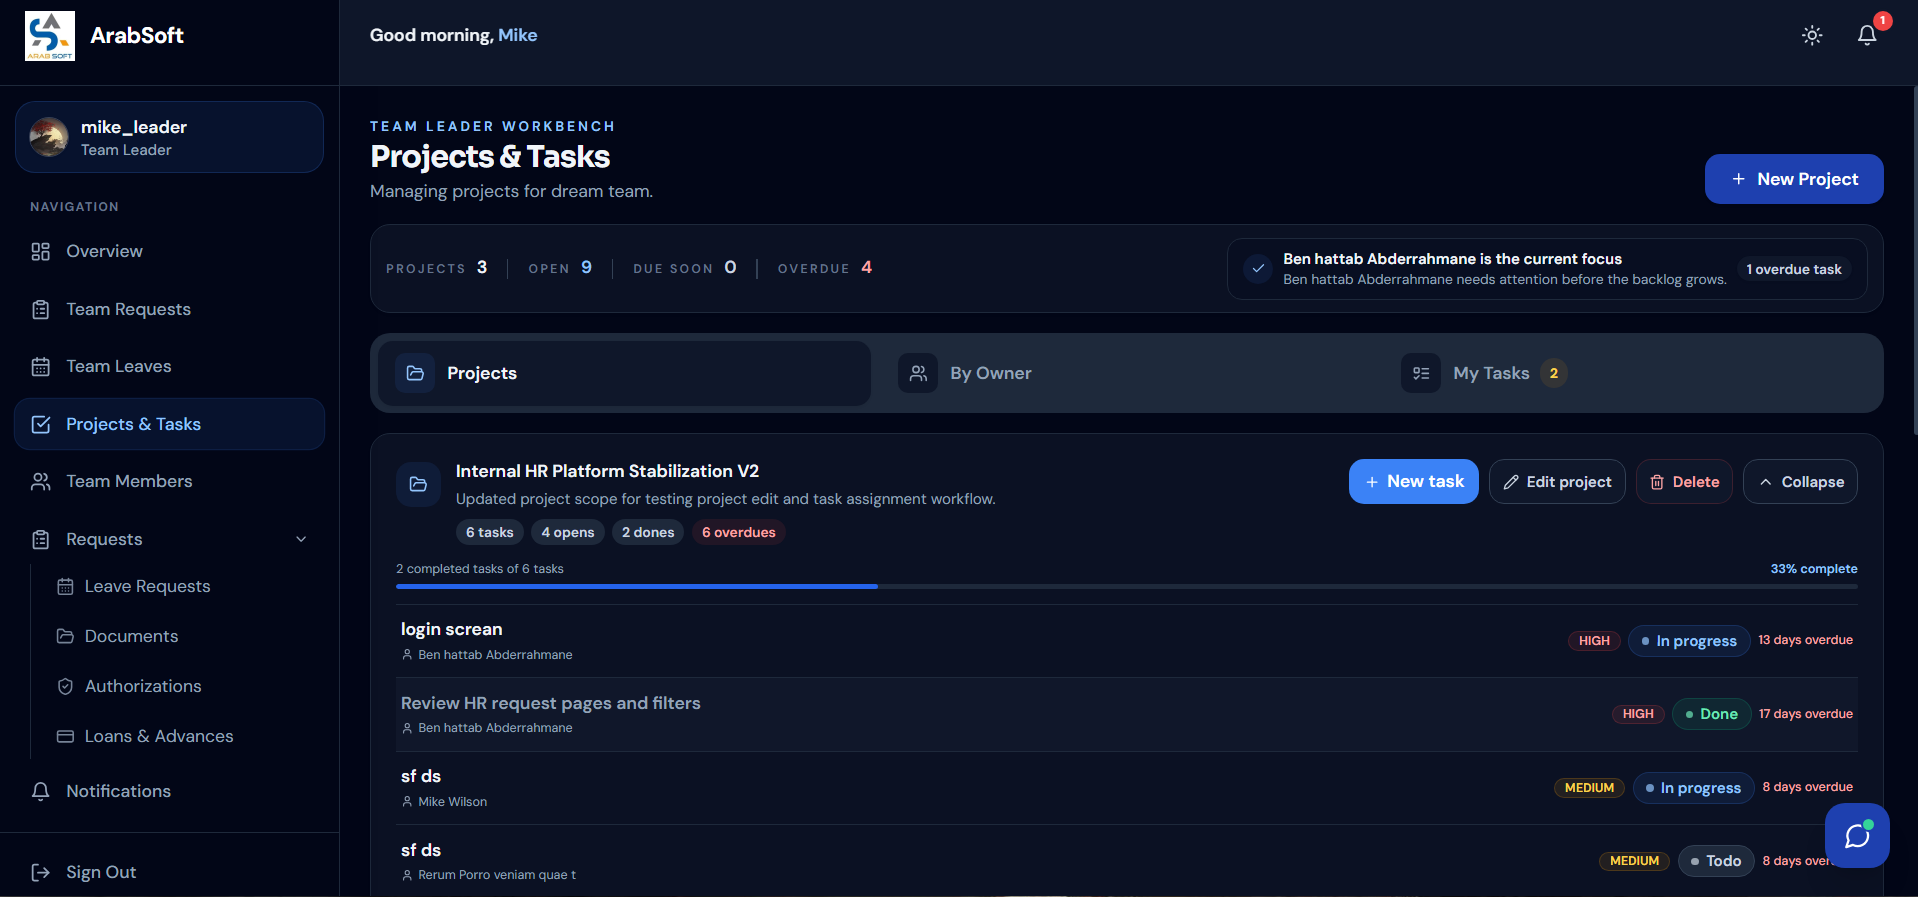
\includegraphics[width=0.95\textwidth,keepaspectratio]{sections/chapitre5/img/sprint5_projects_tasks_reports/09_ui_screenshots/sprint5_team_projects_page.png}
    \caption{Team Projects and Tasks Interface}
    \label{fig:sprint5_team_projects_ui}
  \end{figure}

  \Needspace{12cm}
  \begin{figure}[H]
    \centering
    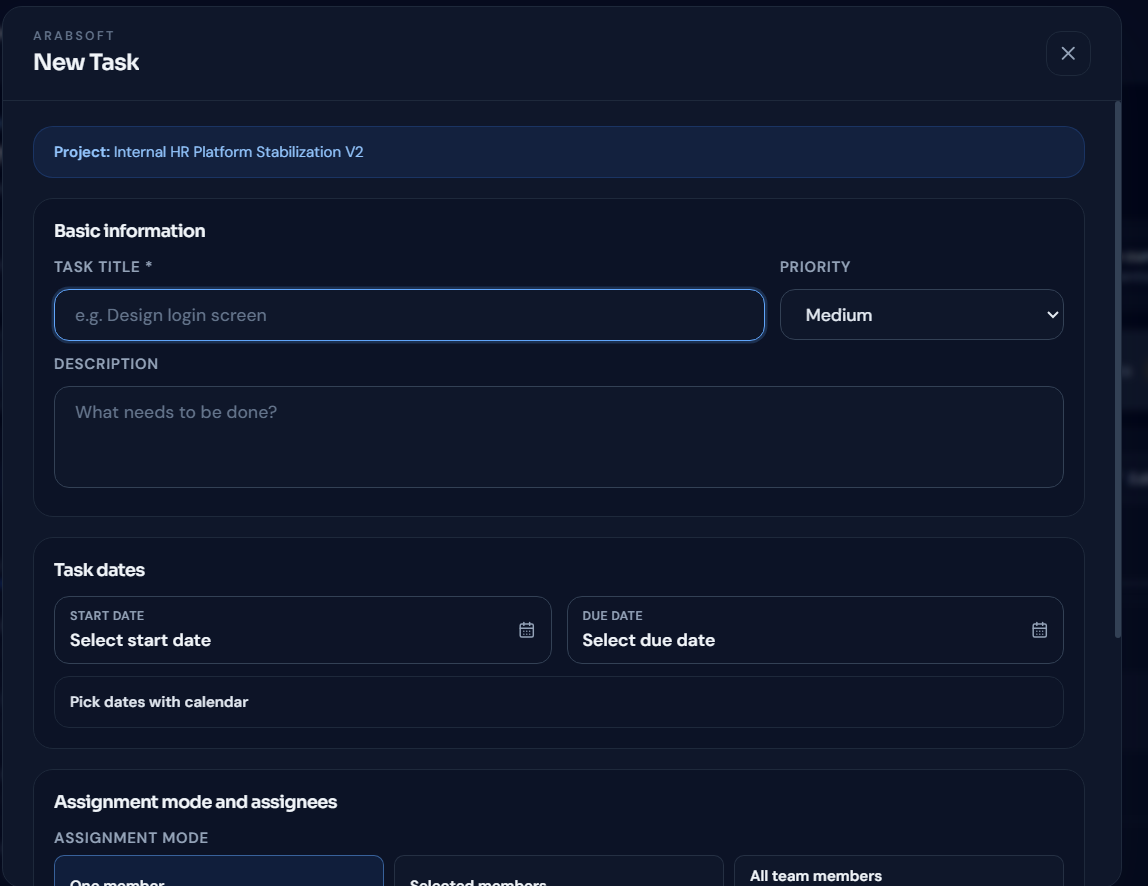
\includegraphics[width=0.95\textwidth,keepaspectratio]{sections/chapitre5/img/sprint5_projects_tasks_reports/09_ui_screenshots/sprint5_task_assignment_modal1.png}
    \vspace{0.05cm}
    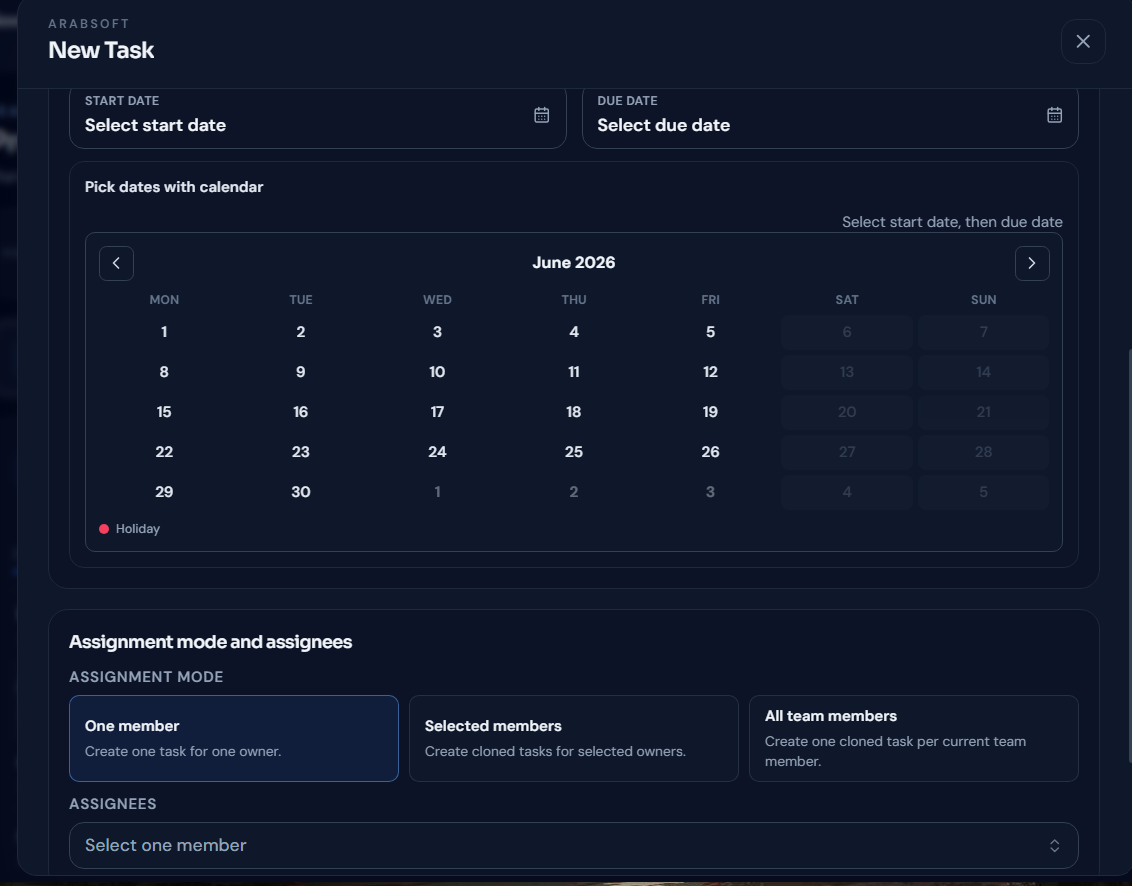
\includegraphics[width=0.95\textwidth,keepaspectratio]{sections/chapitre5/img/sprint5_projects_tasks_reports/09_ui_screenshots/sprint5_task_assignment_modal2.png}
    \caption{Task Assignment Interface}
    \label{fig:sprint5_task_assignment_ui}
  \end{figure}

  \Needspace{12cm}
  \begin{figure}[H]
    \centering
    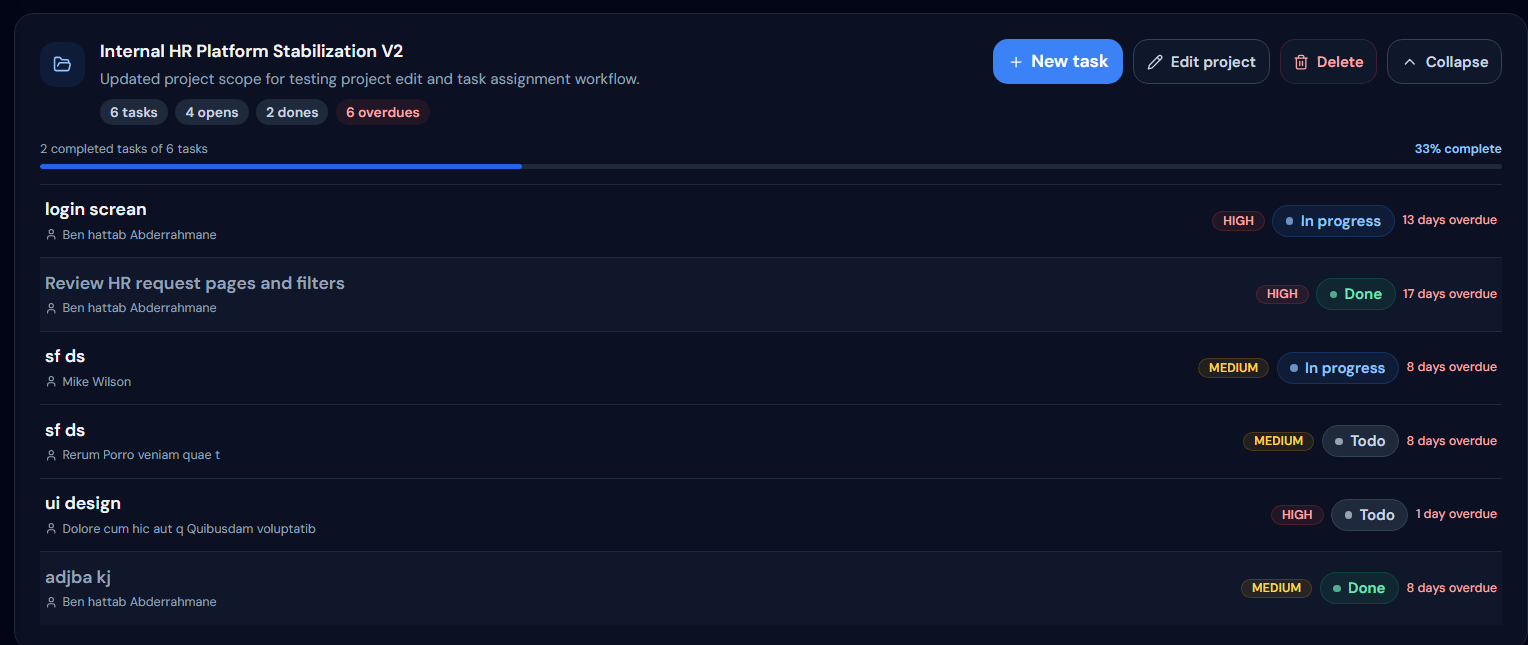
\includegraphics[width=0.95\textwidth,keepaspectratio]{sections/chapitre5/img/sprint5_projects_tasks_reports/09_ui_screenshots/sprint5_employee_tasks_page.png}
    \vspace{0.05cm}
    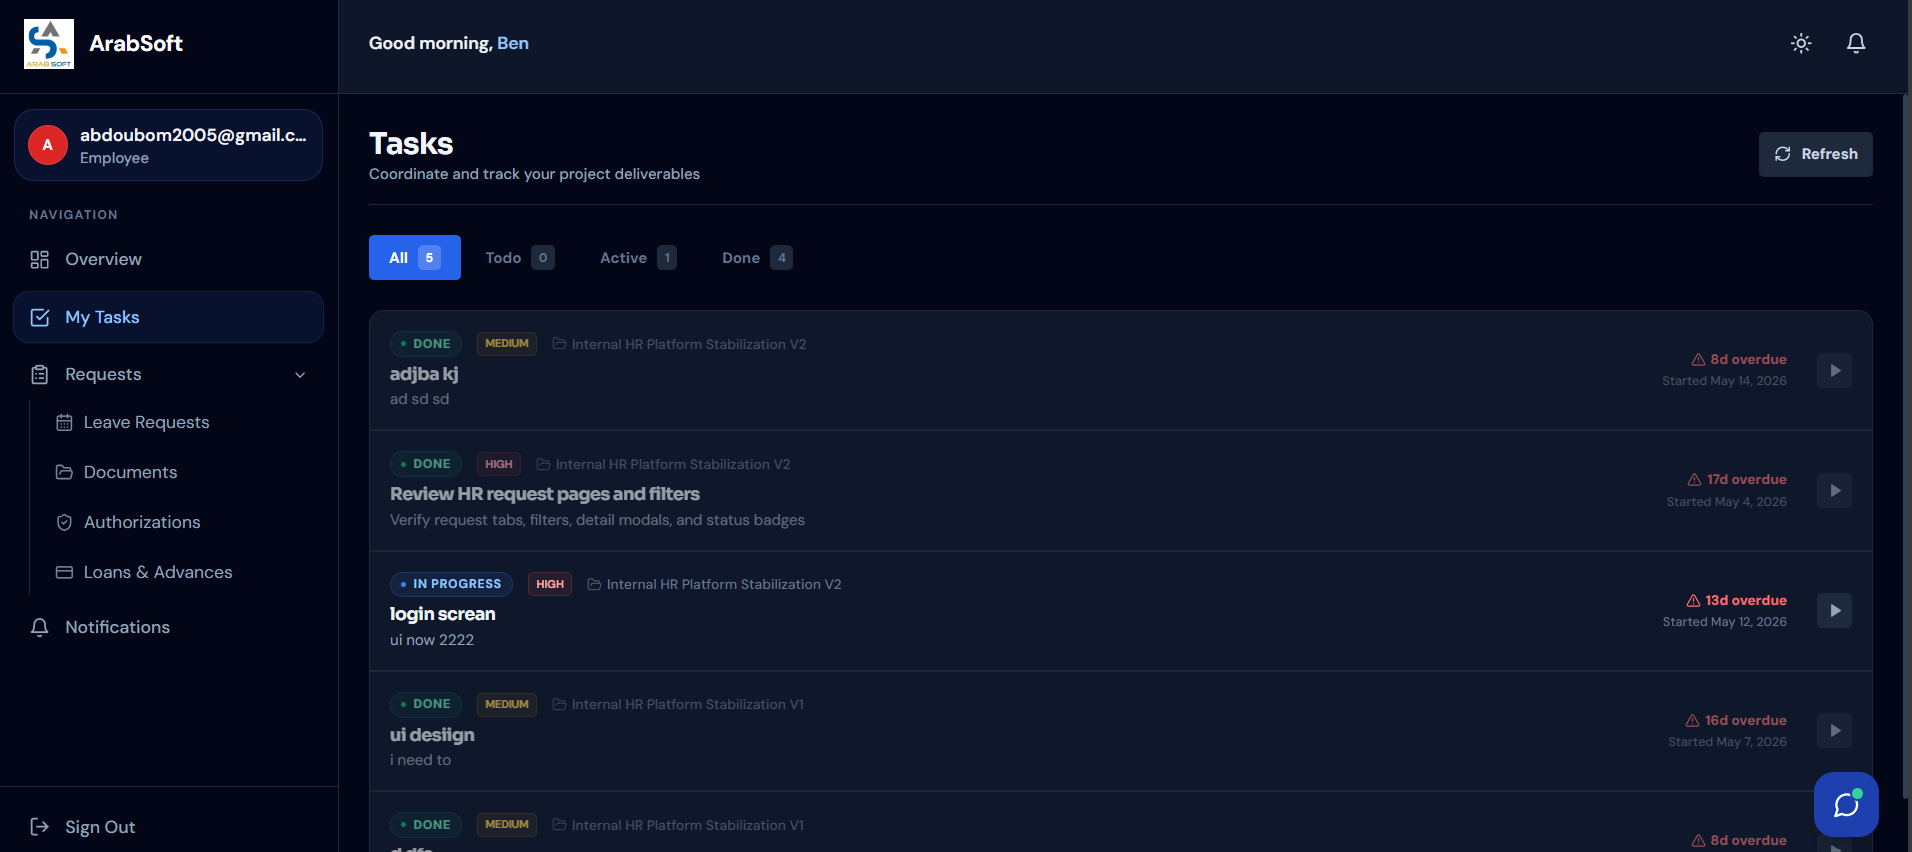
\includegraphics[width=0.95\textwidth,keepaspectratio]{sections/chapitre5/img/sprint5_projects_tasks_reports/09_ui_screenshots/sprint5_employee_tasks_page emp side.png}
    \caption{Employee Task Tracking Interface}
    \label{fig:sprint5_employee_tasks_ui}
  \end{figure}

  \Needspace{7.2cm}
  \begin{figure}[H]
    \centering
    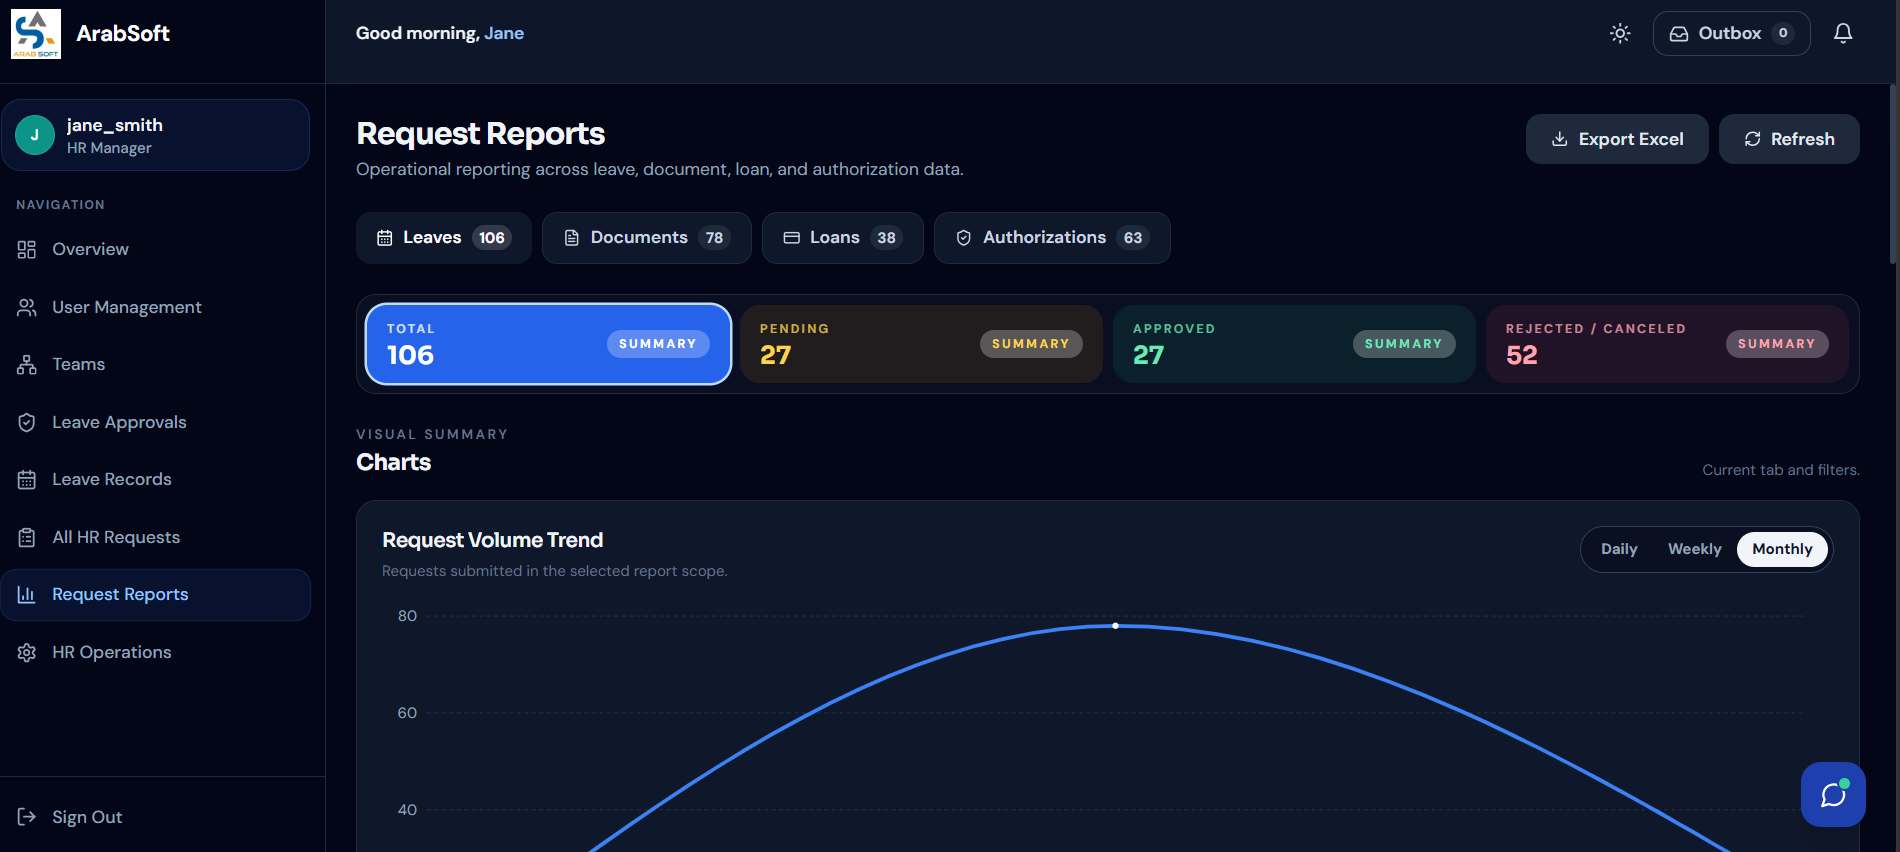
\includegraphics[width=0.95\textwidth,keepaspectratio]{sections/chapitre5/img/sprint5_projects_tasks_reports/09_ui_screenshots/sprint5_hr_reports_page1.png}
    \caption{HR Request Reports Interface}
    \label{fig:sprint5_hr_reports_ui}
  \end{figure}

  \Needspace{12cm}
  \begin{figure}[H]
    \centering
    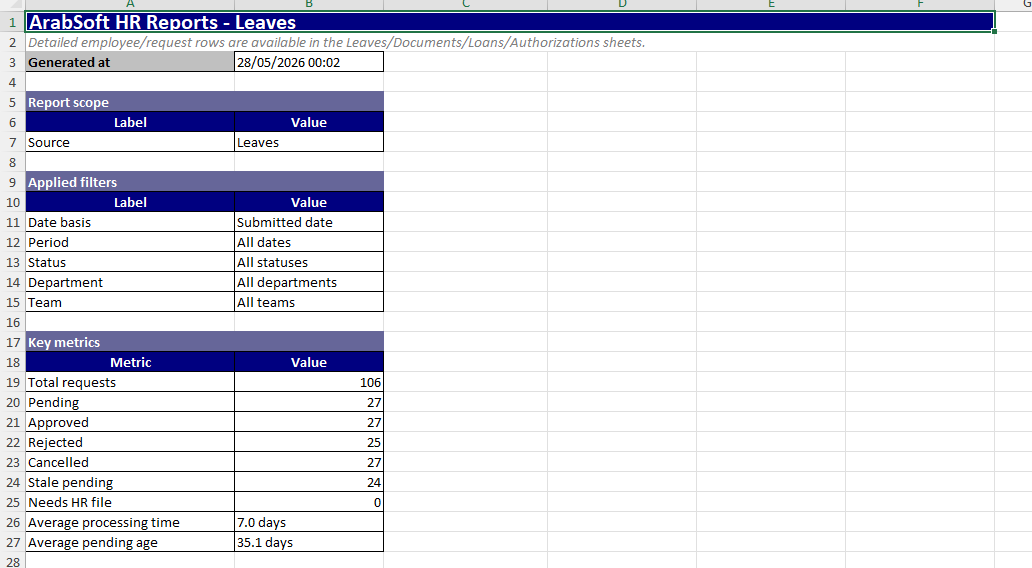
\includegraphics[width=0.95\textwidth,keepaspectratio]{sections/chapitre5/img/sprint5_projects_tasks_reports/09_ui_screenshots/res 1.png}
    \vspace{0.05cm}
    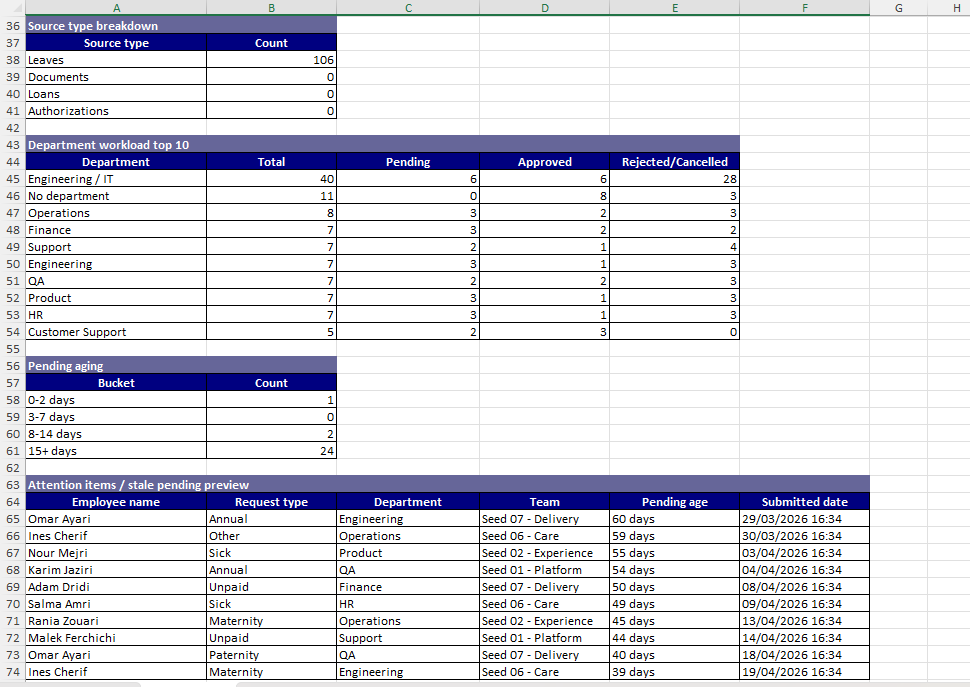
\includegraphics[width=0.95\textwidth,keepaspectratio]{sections/chapitre5/img/sprint5_projects_tasks_reports/09_ui_screenshots/res 2.png}
    \caption{Excel Report Export Result}
    \label{fig:sprint5_excel_export_result_ui}
  \end{figure}

  \ReportSubsection{II.5 Sprint Review}{\hspace{0.5cm} 5. Sprint Review}

  {\fontsize{12}{18}\selectfont
  \setlength{\parindent}{1.2cm}
  \setlength{\parskip}{6pt}

  \indent Sprint 5 delivered team-scoped project management, task assignment with availability checks, task status tracking by assignees, and HR report consultation with Excel export. Team leaders can manage projects and tasks in one place, and HR managers can filter and export administrative request data.

  }

\ReportSubsection{II.6 Sprint Retrospective}{\hspace{0.5cm} 6. Sprint Retrospective}

\begin{table}[H]
\centering
\renewcommand{\arraystretch}{1.7}
\setlength{\tabcolsep}{8pt}
\begin{tabular}{|>{\RaggedRight\arraybackslash}m{6.2cm}|>{\RaggedRight\arraybackslash}m{6.2cm}|}
\hline
\rowcolor{blue!20}
\centering\textbf{What went well} & \centering\textbf{What needs improvement} \tabularnewline
\hline
The sprint turned team work into a complete flow: team leaders can manage projects, assign tasks with different modes, and assignees can follow task progress through a clear lifecycle.
&
Task assignment became the most sensitive part of the sprint because team scope, member availability, assignment modes, and validation feedback all had to stay consistent.
\\
\hline
HR reporting became more useful through filters and Excel export, allowing administrative request data to be reviewed outside the platform.
&
Future reporting should be expanded carefully: project and task analytics should only be added when a dedicated and reliable backend source exists.
\\
\hline
\end{tabular}
\caption{Sprint Retrospective -- Sprint 5}
\label{tab:sprint5_retrospective}
\end{table}

  % ============================================================
  %  III. SPRINT 6: AI ASSISTANT, LOCAL DEPLOYMENT, AND STABILIZATION
  % ============================================================
  \ReportSection{III. Sprint 6: AI Assistant, Local Deployment, and Stabilization}{III. Sprint 6: AI Assistant, Local Deployment, and Stabilization}

  \ReportSubsection{III.1 Sprint Goal}{\hspace{0.5cm} 1. Sprint Goal}

  {\fontsize{12}{18}\selectfont
  \setlength{\parindent}{1.2cm}
  \setlength{\parskip}{6pt}

  \indent This sprint focuses on the ArabSoft AI assistant, local deployment packaging, and final stabilization. The assistant is guidance-only, Spring Boot remains the secure gateway, and FastAPI receives only safe context prepared by the backend. \cite{fastapi_docs} Gemini is optional and the deployment scope remains limited to local Docker Compose.

  }

  \ReportSubsection{III.2 Visual Sprint Journal}{\hspace{0.5cm} 2. Visual Sprint Journal}

  {\fontsize{12}{18}\selectfont
  \setlength{\parindent}{1.2cm}
  \setlength{\parskip}{6pt}

  \indent The Sprint 6 visual journal reflects the validated assistant and deployment work completed during the sprint.

  }

  \ReportSubsection{III.3 Sprint Backlog}{\hspace{0.5cm} 3. Sprint Backlog}

  {\fontsize{12}{18}\selectfont
  \setlength{\parindent}{1.2cm}
  \setlength{\parskip}{6pt}

  \indent The table below summarizes the Sprint 6 work packages prepared from the validated implementation scope.

  }

  \begin{table}[H]
  \centering
  \normalsize
  \renewcommand{\arraystretch}{2.05}
  \setlength{\extrarowheight}{5pt}
  \setlength{\tabcolsep}{4pt}
  \begin{tabular}{|>{\centering\bfseries\arraybackslash}m{1.5cm}|>{\centering\bfseries\arraybackslash}m{3.6cm}|>{\RaggedRight\arraybackslash}m{7.4cm}|>{\centering\arraybackslash}m{1.6cm}|}
  \hline
  \rowcolor{blue!20}
  \textbf{Sprint} & \textbf{Stories} & \centering\textbf{Tasks} & \textbf{Duration} \\
  \hline
  \multirow{7}{=}{\centering\textbf{Sprint 6}}
  & \multirow{1}{=}{\centering\textbf{AI assistant platform help and Q\&A}}
  & Route assistant questions through Spring Boot, use role-aware platform guidance, and return safe navigation/help responses.
  & \multirow{1}{=}{\centering 2d} \\
  \cline{2-4}
  & \multirow{1}{=}{\centering\textbf{AI request drafting assistant}}
  & Support leave, document, authorization, and loan drafts with preview, validation, and explicit submission.
  & \multirow{1}{=}{\centering 3d} \\
  \cline{2-4}
  & \multirow{1}{=}{\centering\textbf{Team Leader decision support}}
  & Provide read-only decision support for one selected leave request using safe team and workload context.
  & \multirow{1}{=}{\centering 2d} \\
  \cline{2-4}
  & \multirow{1}{=}{\centering\textbf{Assistant safety and role restrictions}}
  & Enforce refusal rules, sanitize routes, protect against stale confirmations, and keep the assistant guidance-only.
  & \multirow{1}{=}{\centering 2d} \\
  \cline{2-4}
  & \multirow{1}{=}{\centering\textbf{Assistant UI rendering}}
  & Render assistant replies, draft previews, and decision-support cards in the frontend.
  & \multirow{1}{=}{\centering 2d} \\
  \cline{2-4}
  & \multirow{1}{=}{\centering\textbf{Local Docker deployment}}
  & Containerize the frontend, backend, AI service, PostgreSQL, Keycloak, Kafka, Zookeeper, and PgAdmin for local deployment and testing.
  & \multirow{1}{=}{\centering 2d} \\
  \cline{2-4}
  & \multirow{1}{=}{\centering\textbf{Stabilization and regression coverage}}
  & Keep fallback paths, safety checks, and assistant regression tests aligned with the implemented behavior.
  & \multirow{1}{=}{\centering 1d} \\
  \hline
  \end{tabular}
  \caption*{Sprint Backlog -- Sprint 6}
  \phantomsection\label{tab:sprint6_backlog}
  \end{table}

  \clearpage
  \ReportSubsection{III.4 Requirements Analysis}{\hspace{0.5cm} 4. Requirements Analysis}

  {\fontsize{12}{18}\selectfont
  \setlength{\parindent}{1.2cm}
  \setlength{\parskip}{6pt}

  \indent Sprint 6 adds an assistant scope centered on guidance, request drafting, and decision support. The assistant helps users ask platform questions, prepare drafts, review validation feedback, and access suggested pages. Final workflow decisions remain with the user and the authorized role.

  }

  \ReportSubsubsection{Assistant Scope and Business Rules}

  {\fontsize{12}{18}\selectfont
  \setlength{\parindent}{1.2cm}
  \setlength{\parskip}{6pt}

  \indent Figure~\ref{fig:sprint6_ai_assistant_decision_support_use_case} summarizes the user-facing assistant scope for Sprint 6. It covers platform questions, request drafting, validation preview, suggested pages, and Team Leader decision support. The assistant remains guidance-only and does not take workflow decisions.

  }

  \Needspace{10\baselineskip}
  \begin{figure}[H]
    \centering
    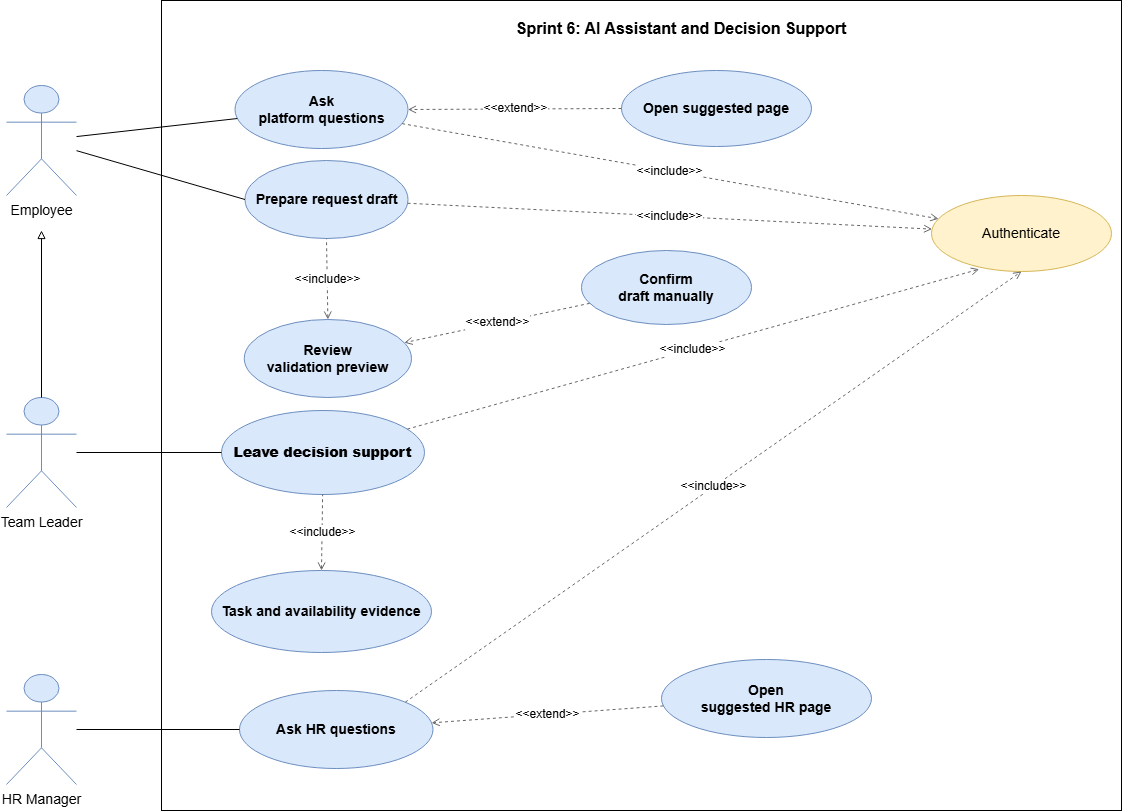
\includegraphics[width=0.95\textwidth,keepaspectratio]{sections/chapitre5/img/sprint6_ai_deployment_stabilization/02_use_case_diagrams/use_case_sprint6_ai_assistant_decision_support.png}
    \caption{Use Case Diagram -- Sprint 6 AI Assistant and Decision Support}
    \label{fig:sprint6_ai_assistant_decision_support_use_case}
  \end{figure}

  {\fontsize{12}{18}\selectfont
  \setlength{\parindent}{1.2cm}
  \setlength{\parskip}{6pt}

  \indent The assistant remains focused on safe guidance and manual control. It does not approve, reject, submit, or change roles on behalf of the user.

  }

  \ReportSubsubsection{System Sequence Diagrams}

  {\fontsize{12}{18}\selectfont
  \setlength{\parindent}{1.2cm}
  \setlength{\parskip}{6pt}

  \indent The Sprint 6 system sequence diagrams describe the user-system interaction for assistant access, request drafting, and Team Leader decision support. The assistant remains guidance-only and does not take workflow decisions.

  }

  \Needspace{7.2cm}
  \begin{figure}[H]
    \centering
    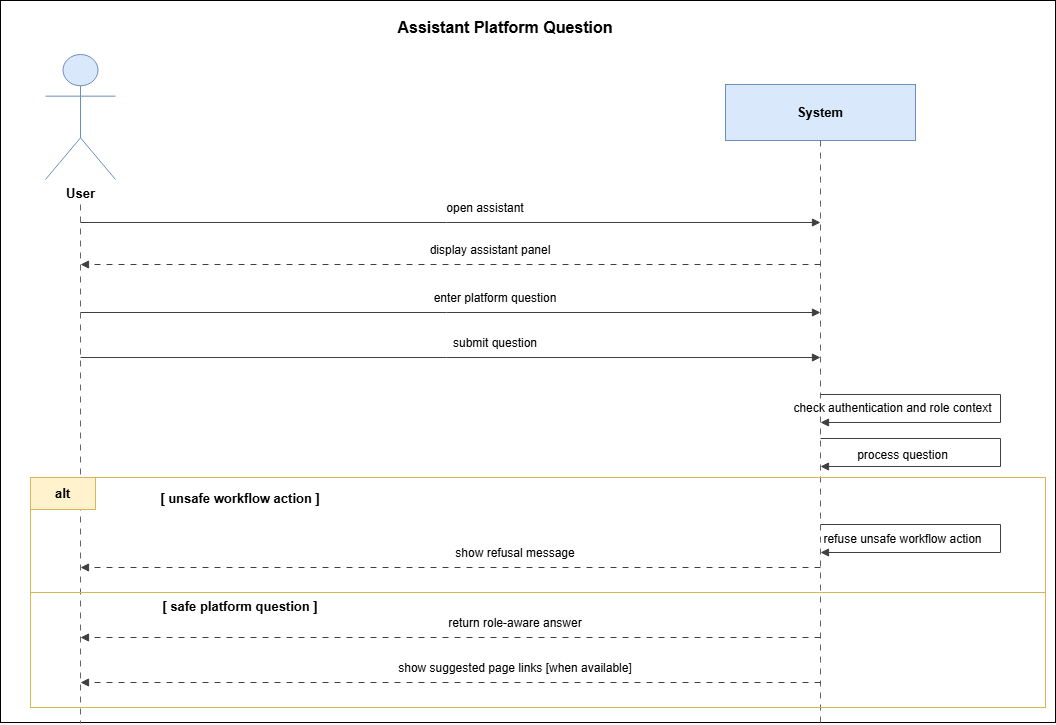
\includegraphics[width=0.95\textwidth,keepaspectratio]{sections/chapitre5/img/sprint6_ai_deployment_stabilization/03_system_sequence_diagrams/ssd_assistant_platform_question.png}
    \caption{System Sequence Diagram -- Assistant Platform Question}
    \label{fig:sprint6_ssd_assistant_platform_question}
  \end{figure}

  \Needspace{7.2cm}
  \begin{figure}[H]
    \centering
    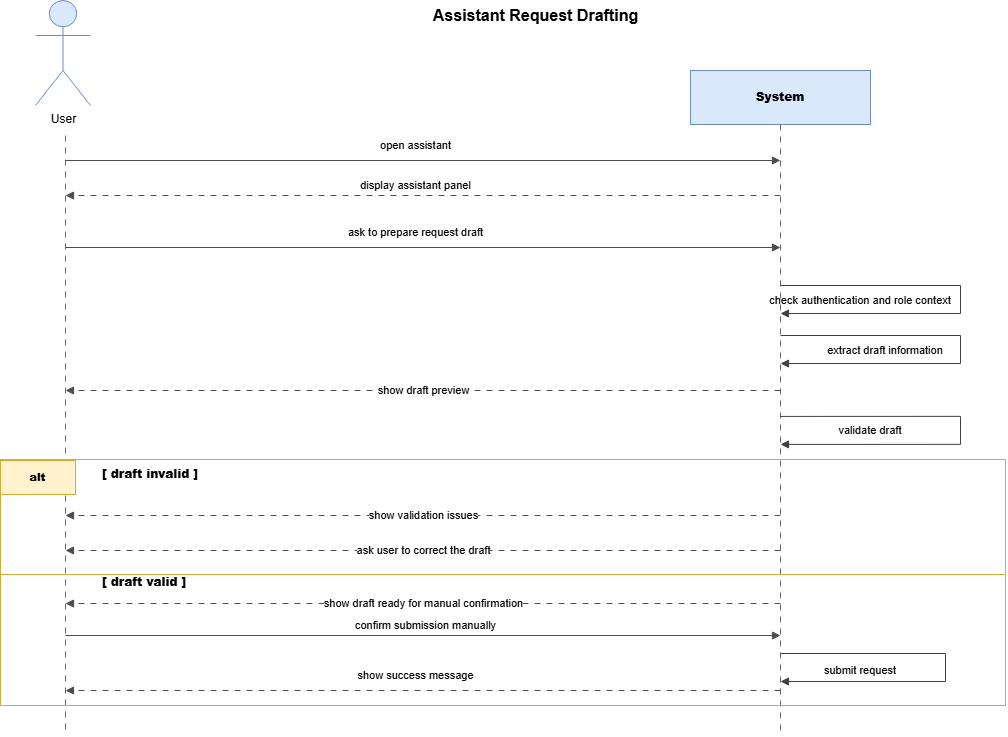
\includegraphics[width=0.95\textwidth,keepaspectratio]{sections/chapitre5/img/sprint6_ai_deployment_stabilization/03_system_sequence_diagrams/ssd_assistant_request_drafting.png}
    \caption{System Sequence Diagram -- Assistant Request Drafting}
    \label{fig:sprint6_ssd_assistant_request_drafting}
  \end{figure}

  \Needspace{7.2cm}
  \begin{figure}[H]
    \centering
    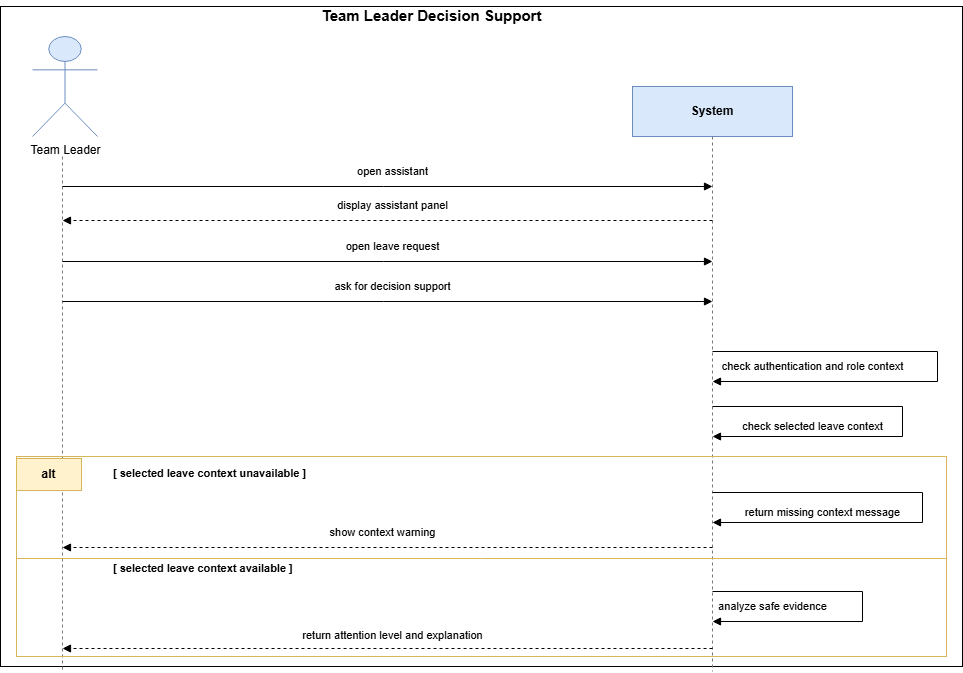
\includegraphics[width=0.95\textwidth,keepaspectratio]{sections/chapitre5/img/sprint6_ai_deployment_stabilization/03_system_sequence_diagrams/ssd_team_leader_decision_support.png}
    \caption{System Sequence Diagram -- Team Leader Decision Support}
    \label{fig:sprint6_ssd_team_leader_decision_support}
  \end{figure}

  \ReportSubsubsection{Analysis and Design Decisions}

  {\fontsize{12}{18}\selectfont
  \setlength{\parindent}{1.2cm}
  \setlength{\parskip}{6pt}

  \indent Sprint 6 is documented with three complementary views: the domain model for the assistant context data, the participant class view for the gateway interaction, and the design class view for the safe assistant structures. Together, these diagrams separate persistent domain data from the assistant-specific object structure.

  }

  \ReportSubsubsection{Domain Model}

  {\fontsize{12}{18}\selectfont
  \setlength{\parindent}{1.2cm}
  \setlength{\parskip}{6pt}

  \indent The domain model below shows the real Spring Boot entities used to build the assistant context.

  }

  \Needspace{9\baselineskip}
  \begin{figure}[H]
    \centering
    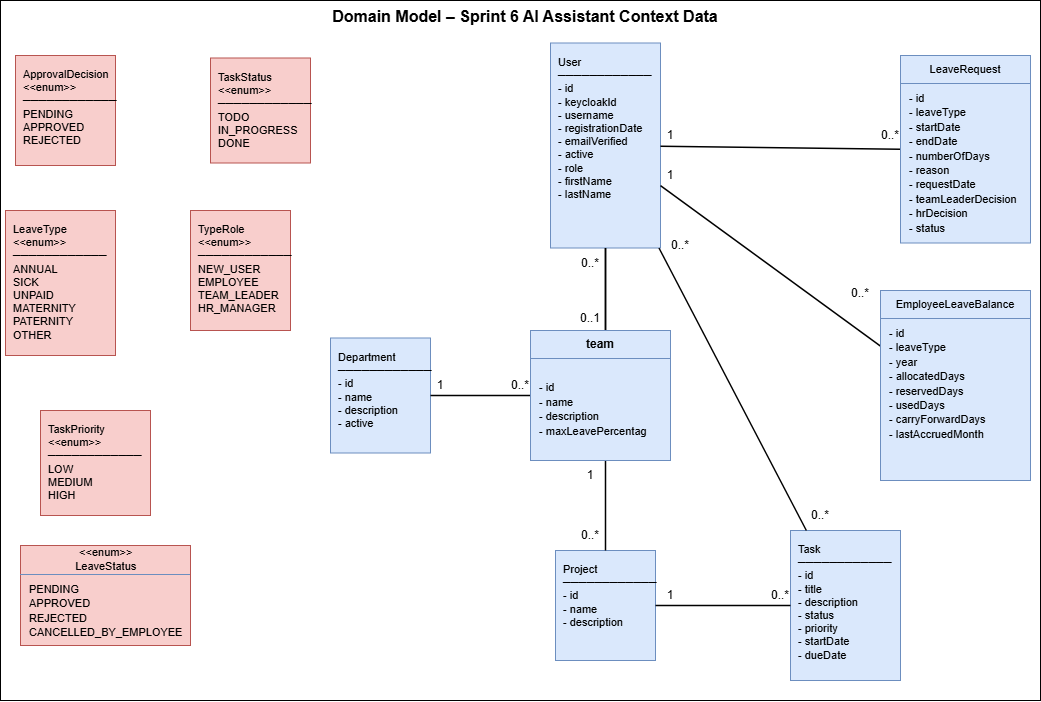
\includegraphics[width=0.95\textwidth,keepaspectratio]{sections/chapitre5/img/sprint6_ai_deployment_stabilization/05_domain_model/domain_model_sprint6_ai_assistant_context_data.png}
    \caption{Domain Model -- Sprint 6 AI Assistant Context Data}
    \label{fig:sprint6_domain_model_ai_assistant_context_data}
  \end{figure}

  \ReportSubsubsection{Participant Class Diagrams}

  {\fontsize{12}{18}\selectfont
  \setlength{\parindent}{1.2cm}
  \setlength{\parskip}{6pt}

  \indent The participant class diagram below captures the assistant gateway and the safe context contract used during the Sprint 6 assistant flow.

  }

  \Needspace{9\baselineskip}
  \begin{figure}[H]
    \centering
  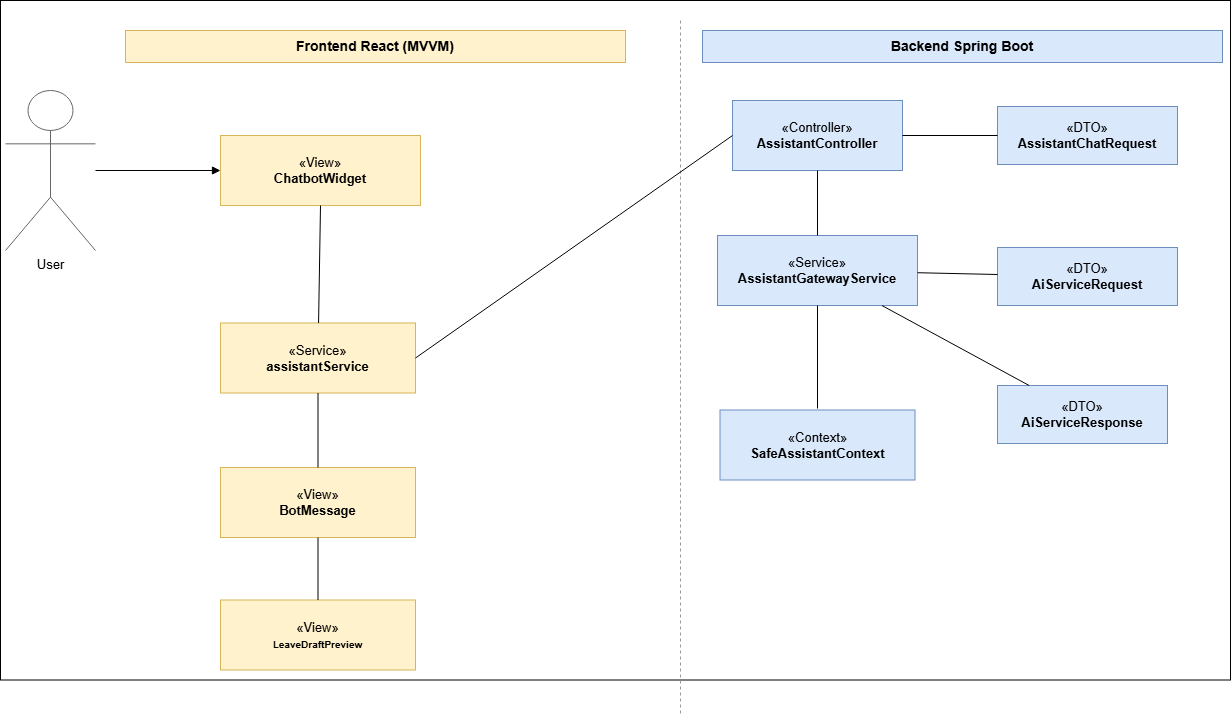
\includegraphics[width=0.95\textwidth,keepaspectratio]{sections/chapitre5/img/sprint6_ai_deployment_stabilization/06_participant_class_diagrams/participant_ai_assistant_gateway_safe_context.png}
    \caption{Participant Class Diagram -- AI Assistant Gateway and Safe Context}
    \label{fig:sprint6_participant_ai_assistant_gateway_safe_context}
  \end{figure}

  \ReportSubsubsection{Design Class Diagrams}

  {\fontsize{12}{18}\selectfont
  \setlength{\parindent}{1.2cm}
  \setlength{\parskip}{6pt}

  \indent The design class diagram below presents the assistant gateway and safe context classes used by the backend implementation.

  }

  \Needspace{9\baselineskip}
  \begin{figure}[H]
    \centering
  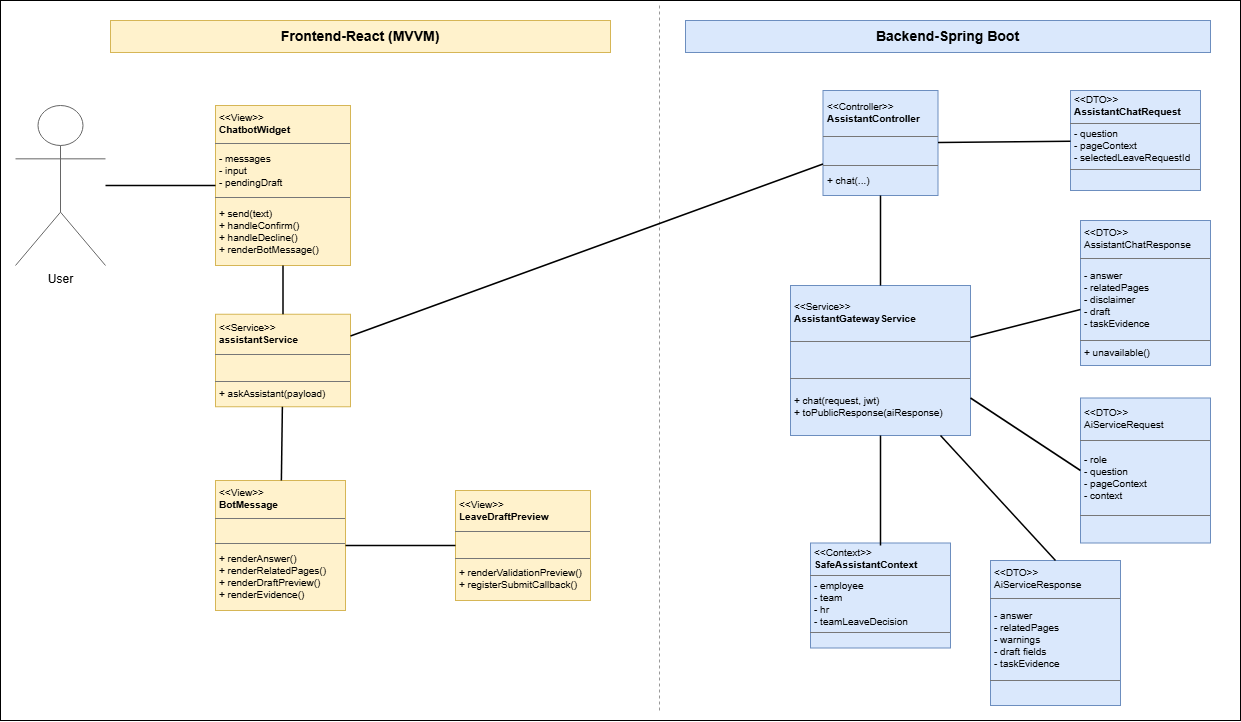
\includegraphics[width=0.95\textwidth,keepaspectratio]{sections/chapitre5/img/sprint6_ai_deployment_stabilization/07_design_class_diagrams/design_ai_assistant_gateway_safe_context.png}
    \caption{Design Class Diagram -- Assistant Gateway and Safe Context}
    \label{fig:sprint6_design_ai_assistant_gateway_safe_context}
  \end{figure}

  \ReportSubsubsection{Conception Sequence Diagrams}

  {\fontsize{12}{18}\selectfont
  \setlength{\parindent}{1.2cm}
  \setlength{\parskip}{6pt}

  \indent The Sprint 6 conception sequence diagrams describe the frontend and backend realization of the assistant flows. The diagrams keep the assistant guidance-only: user questions, request drafting, and Team Leader decision support remain controlled by the authorized user.

  }

  \Needspace{7.2cm}
  \begin{figure}[H]
    \centering
    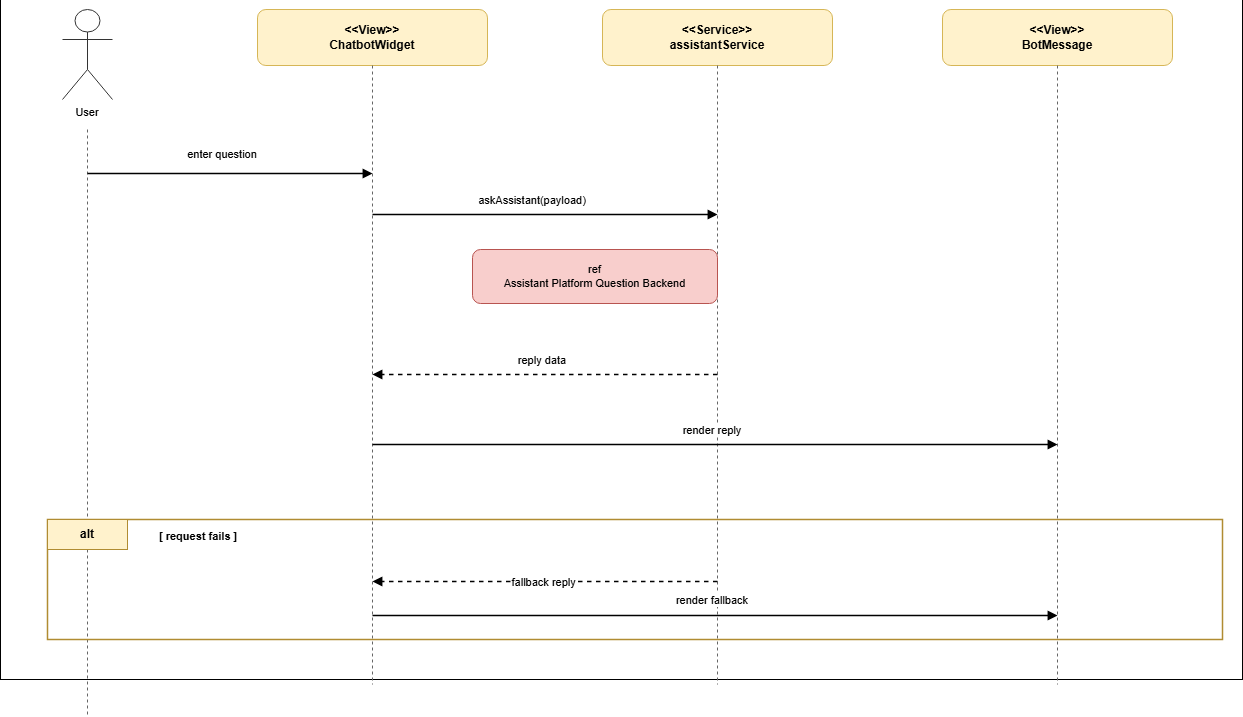
\includegraphics[width=1.0\textwidth,height=0.82\textheight,keepaspectratio]{sections/chapitre5/img/sprint6_ai_deployment_stabilization/08_conception_sequence_diagrams/csd_sprint6_assistant_platform_question_frontend.png}
    \caption{Conception Sequence Diagram -- Assistant Platform Question Frontend}
    \label{fig:sprint6_csd_assistant_platform_question_frontend}
  \end{figure}

  \Needspace{7.2cm}
  \begin{figure}[H]
    \centering
    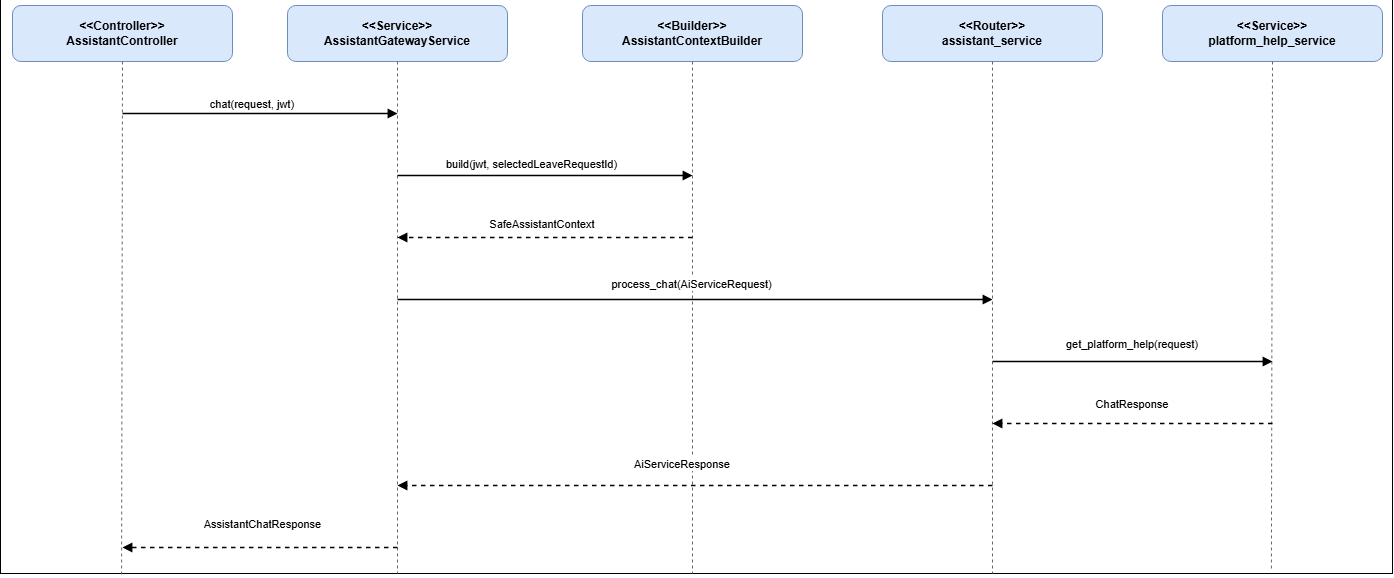
\includegraphics[width=1.0\textwidth,height=0.82\textheight,keepaspectratio]{sections/chapitre5/img/sprint6_ai_deployment_stabilization/08_conception_sequence_diagrams/csd_sprint6_assistant_platform_question_backend.png}
    \caption{Conception Sequence Diagram -- Assistant Platform Question Backend}
    \label{fig:sprint6_csd_assistant_platform_question_backend}
  \end{figure}

  \Needspace{7.2cm}
  \begin{figure}[H]
    \centering
    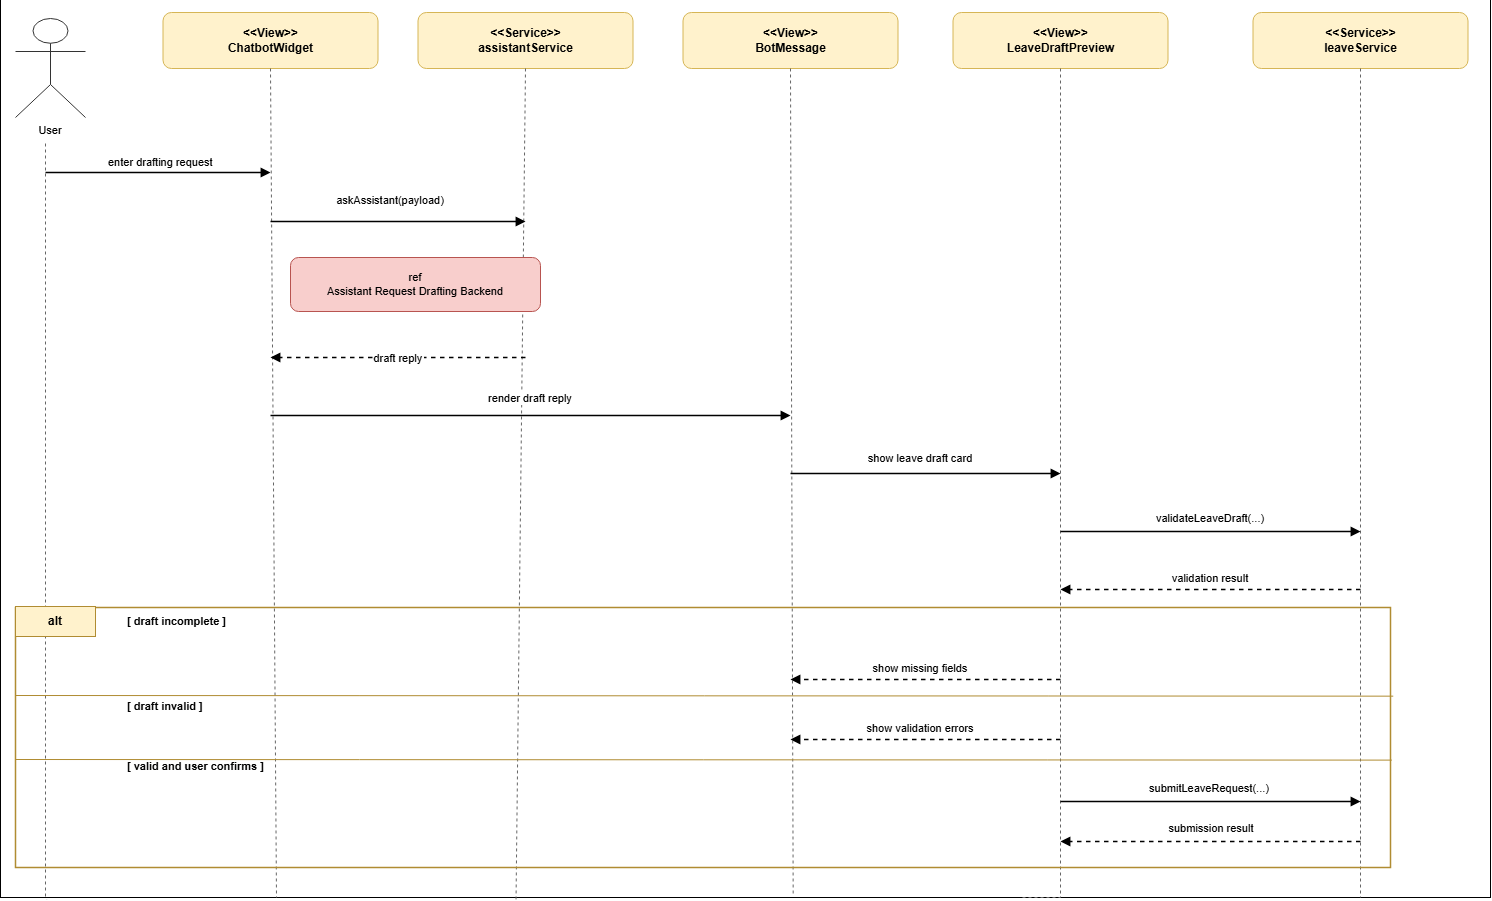
\includegraphics[width=1.0\textwidth,height=0.82\textheight,keepaspectratio]{sections/chapitre5/img/sprint6_ai_deployment_stabilization/08_conception_sequence_diagrams/csd_sprint6_assistant_request_drafting_frontend.png}
    \caption{Conception Sequence Diagram -- Assistant Request Drafting Frontend}
    \label{fig:sprint6_csd_assistant_request_drafting_frontend}
  \end{figure}

  \Needspace{7.2cm}
  \begin{figure}[H]
    \centering
    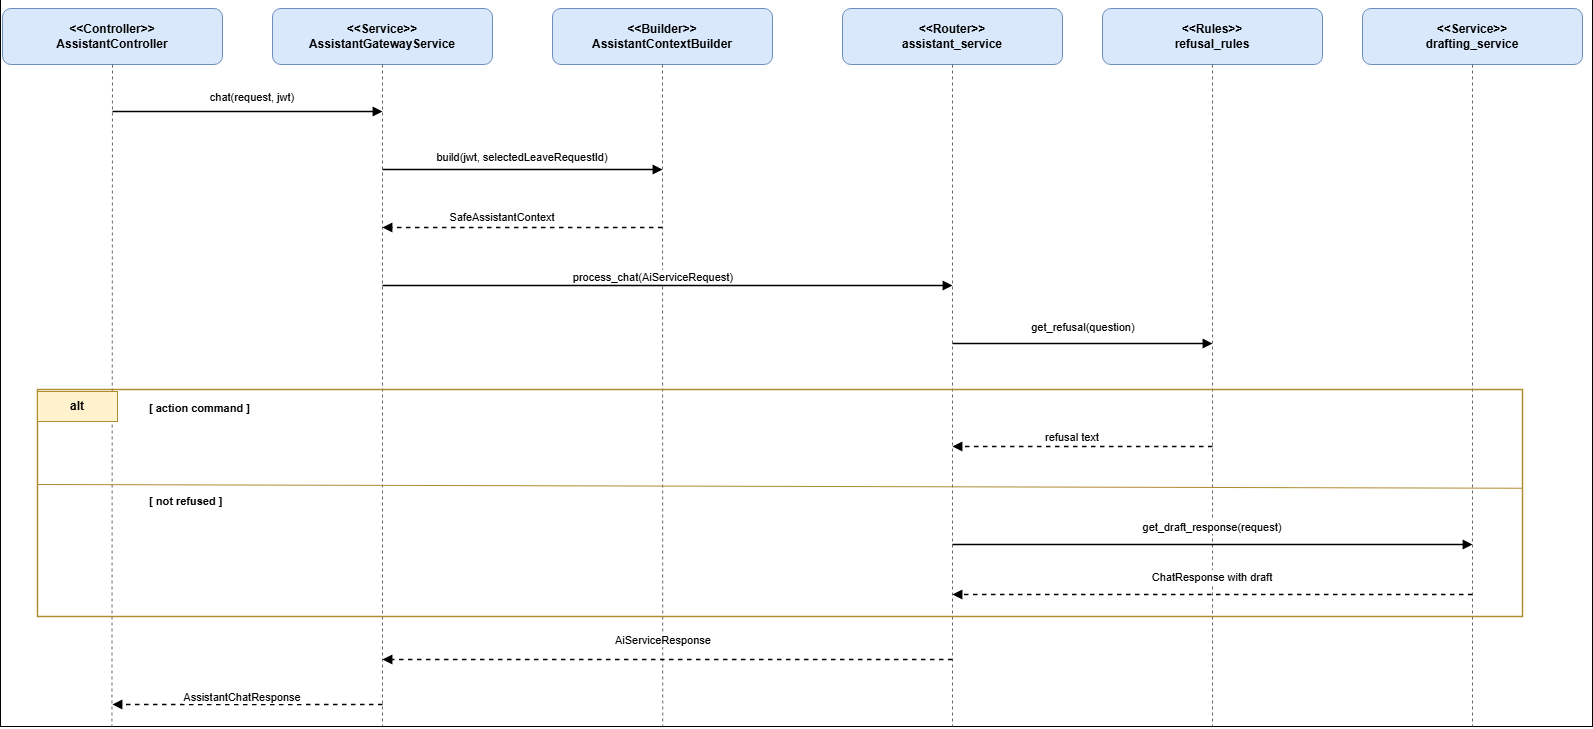
\includegraphics[width=1.0\textwidth,height=0.82\textheight,keepaspectratio]{sections/chapitre5/img/sprint6_ai_deployment_stabilization/08_conception_sequence_diagrams/csd_sprint6_assistant_request_drafting_backend.png}
    \caption{Conception Sequence Diagram -- Assistant Request Drafting Backend}
    \label{fig:sprint6_csd_assistant_request_drafting_backend}
  \end{figure}

  \Needspace{7.2cm}
  \begin{figure}[H]
    \centering
    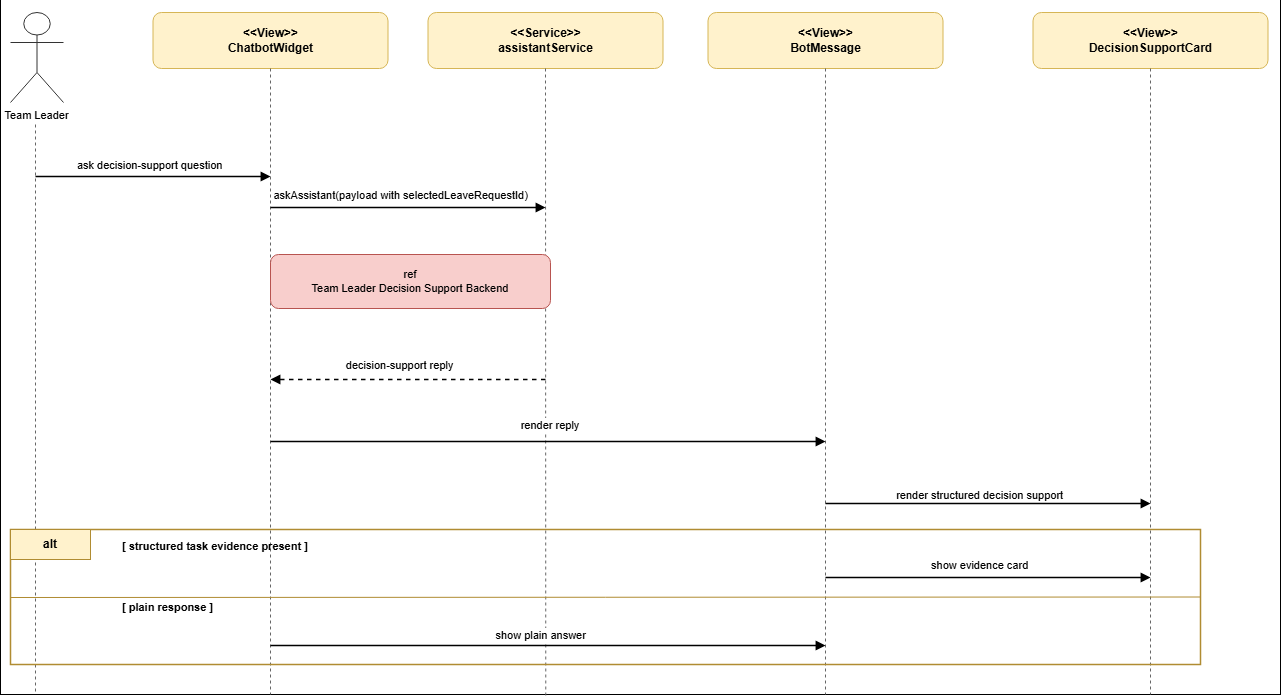
\includegraphics[width=1.0\textwidth,height=0.82\textheight,keepaspectratio]{sections/chapitre5/img/sprint6_ai_deployment_stabilization/08_conception_sequence_diagrams/csd_sprint6_team_leader_decision_support_frontend.png}
    \caption{Conception Sequence Diagram -- Team Leader Decision Support Frontend}
    \label{fig:sprint6_csd_team_leader_decision_support_frontend}
  \end{figure}

  \Needspace{7.2cm}
  \begin{figure}[H]
    \centering
    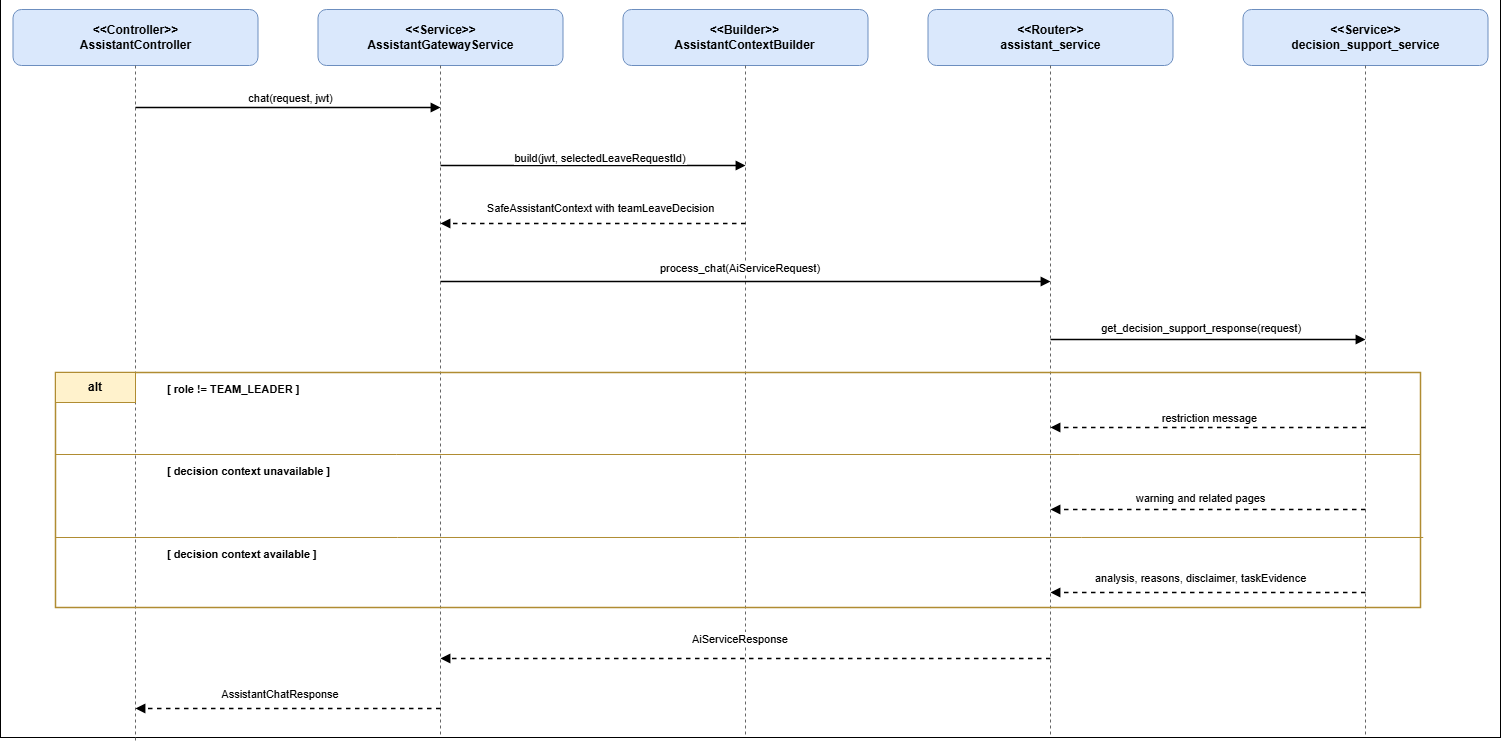
\includegraphics[width=1.0\textwidth,height=0.82\textheight,keepaspectratio]{sections/chapitre5/img/sprint6_ai_deployment_stabilization/08_conception_sequence_diagrams/csd_sprint6_team_leader_decision_support_backend.png}
    \caption{Conception Sequence Diagram -- Team Leader Decision Support Backend}
    \label{fig:sprint6_csd_team_leader_decision_support_backend}
  \end{figure}

  \ReportSubsubsection{Realization}

  {\fontsize{12}{18}\selectfont
  \setlength{\parindent}{1.2cm}
  \setlength{\parskip}{6pt}

  \indent The realization section presents the assistant widget, draft preview cards, decision-support panel, and the local packaging used to validate the sprint scope.

  }

  \ReportSubsubsection{Interface Screenshots}

  {\fontsize{12}{18}\selectfont
  \setlength{\parindent}{1.2cm}
  \setlength{\parskip}{6pt}

  \indent The following screenshots document the Sprint 6 assistant interfaces.

  }

  \Needspace{7.2cm}
  \begin{figure}[H]
    \centering
    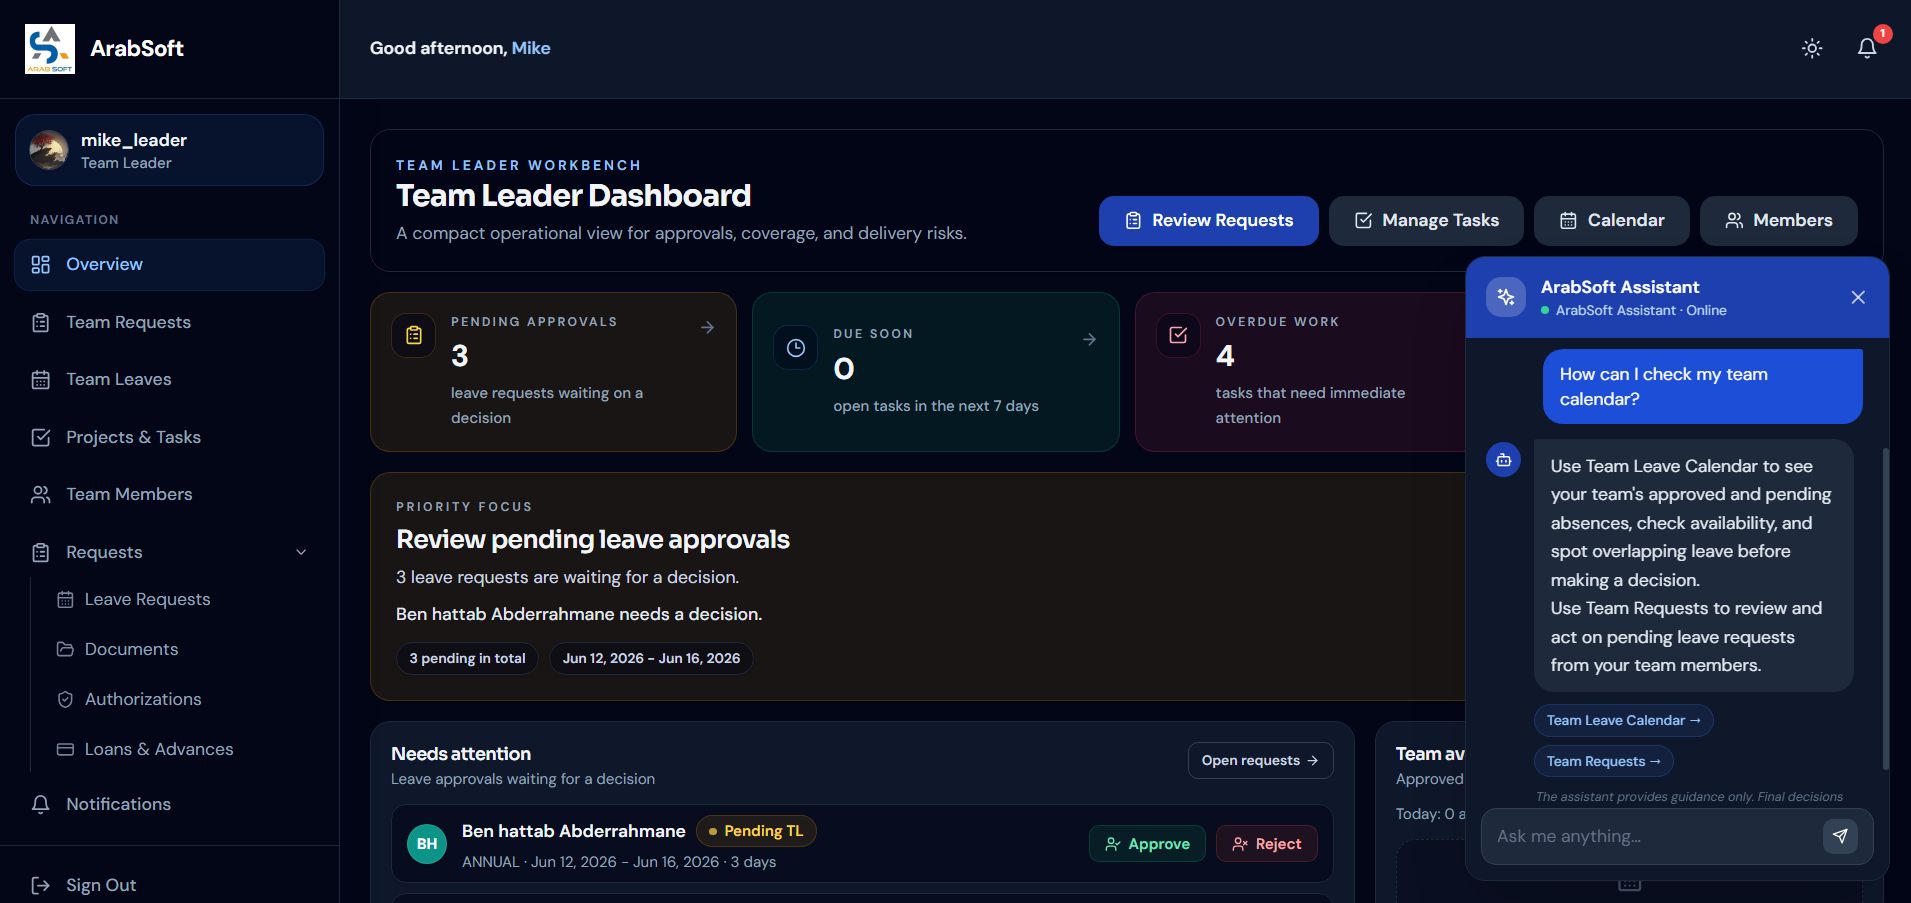
\includegraphics[width=0.95\textwidth,keepaspectratio]{sections/chapitre5/img/sprint6_ai_deployment_stabilization/09_ui_screenshots/sprint6_assistant_platform_qa.png}
    \caption{Assistant Platform Guidance Interface}
    \label{fig:sprint6_assistant_platform_qa_ui}
  \end{figure}

  \Needspace{7.2cm}
  \begin{figure}[H]
    \centering
    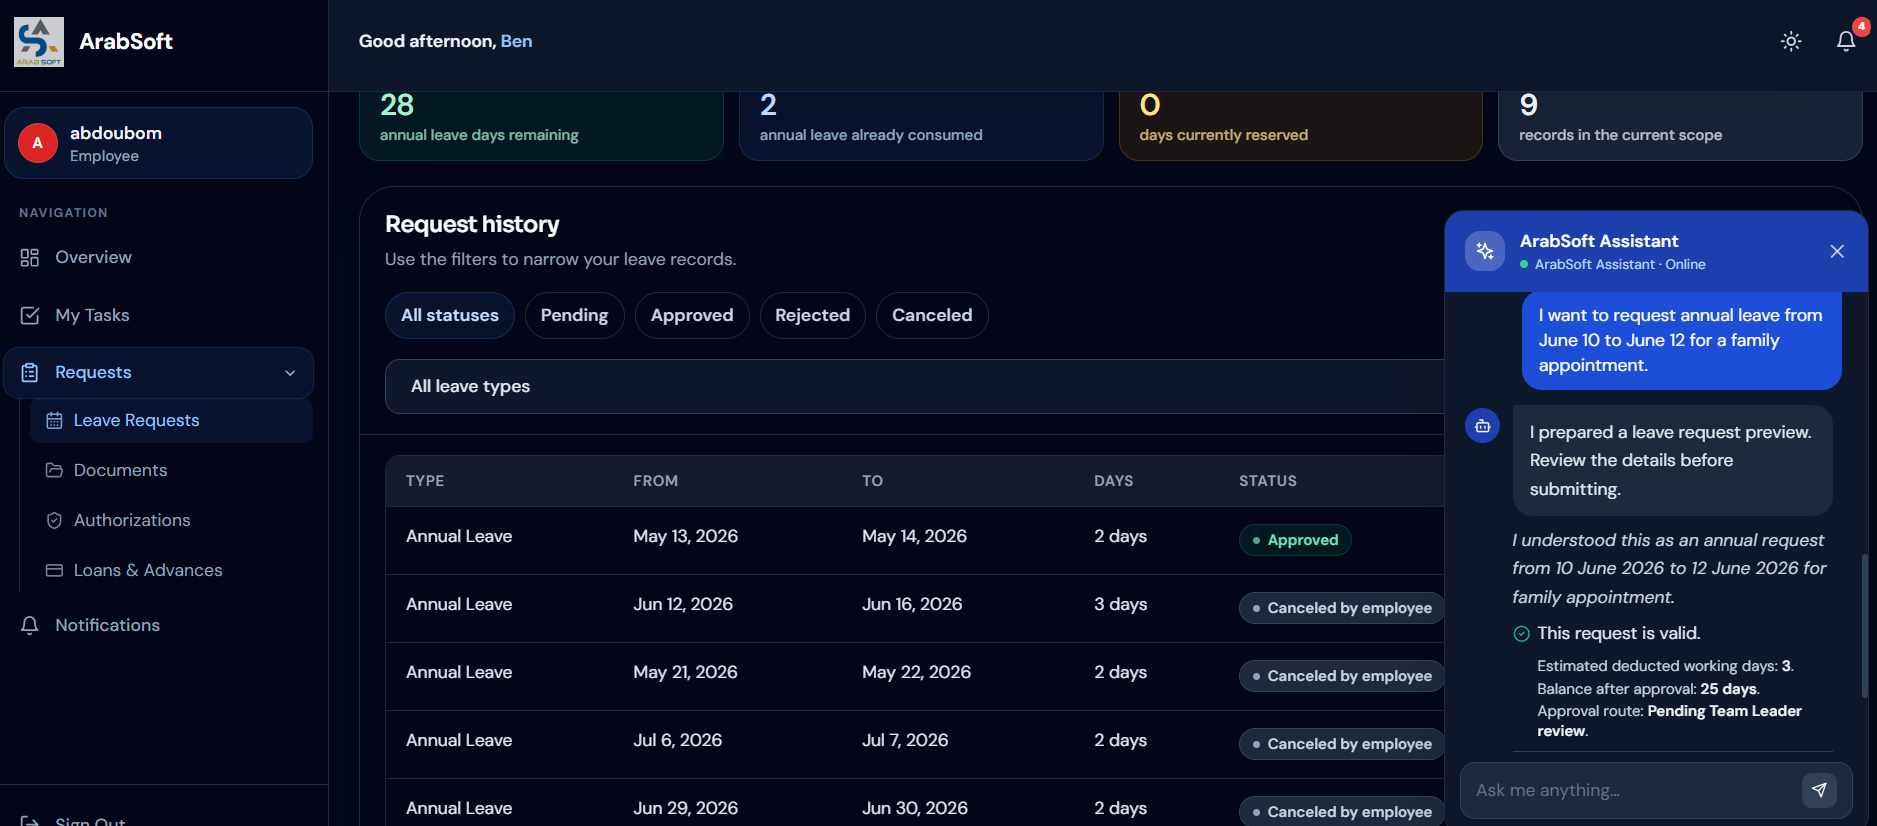
\includegraphics[width=0.95\textwidth,keepaspectratio]{sections/chapitre5/img/sprint6_ai_deployment_stabilization/09_ui_screenshots/sprint6_personal_leave_draft.png}
    \caption{Assistant Leave Draft Preview Interface}
    \label{fig:sprint6_personal_leave_draft_ui}
  \end{figure}

  \Needspace{7.2cm}
  \begin{figure}[H]
    \centering
    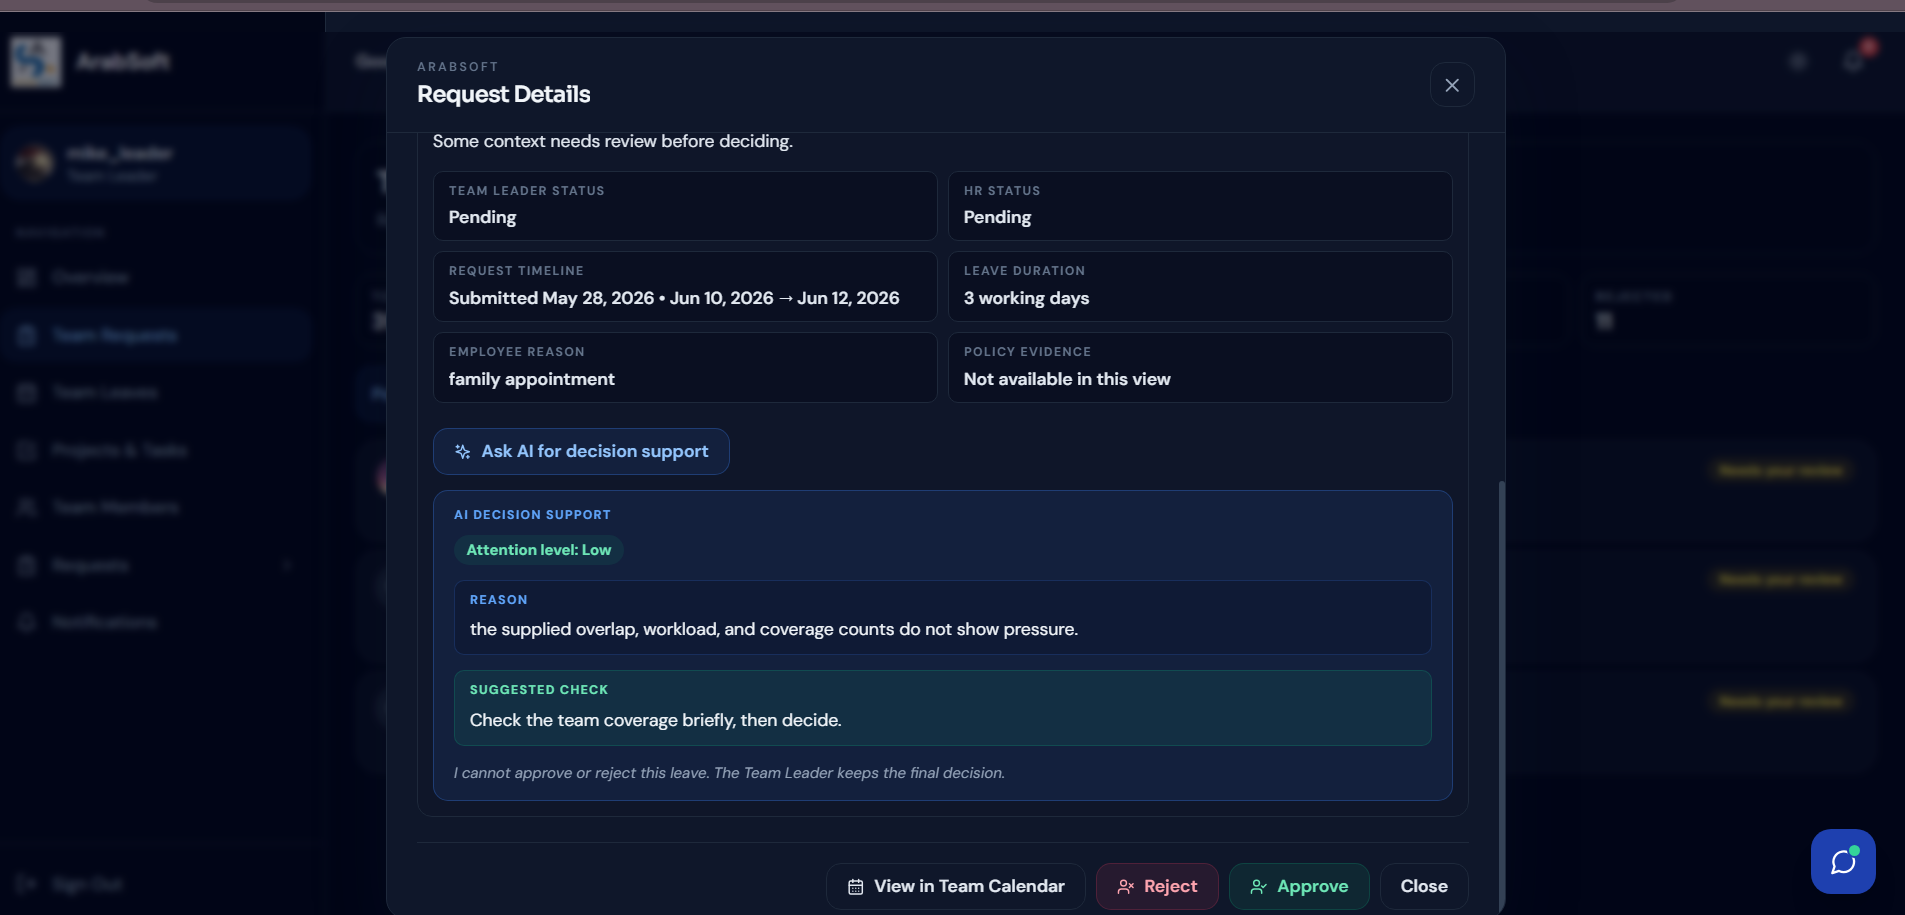
\includegraphics[width=0.95\textwidth,keepaspectratio]{sections/chapitre5/img/sprint6_ai_deployment_stabilization/09_ui_screenshots/sprint6_team_leader_decision_support.png}
    \caption{Team Leader Decision Support Interface}
    \label{fig:sprint6_team_leader_decision_support_ui}
  \end{figure}

  \ReportSubsubsection{Testing and Validation}

  {\fontsize{12}{18}\selectfont
  \setlength{\parindent}{1.2cm}
  \setlength{\parskip}{6pt}

  \indent This section summarizes the regression coverage and safety checks already present in the implementation.

  }

  \ReportSubsection{III.5 Sprint Review}{\hspace{0.5cm} 5. Sprint Review}

  {\fontsize{12}{18}\selectfont
  \setlength{\parindent}{1.2cm}
  \setlength{\parskip}{6pt}

  \indent Sprint 6 completed the assistant scope added in Release 3. The assistant was integrated through the React widget, Spring Boot gateway, and FastAPI AI service. \cite{fastapi_docs} It supports platform questions, request-draft preparation, draft validation preview, suggested page navigation, unsafe-action refusal, and Team Leader decision-support guidance. The review confirmed that the assistant remains guidance-only: it does not approve, reject, submit, cancel, change roles, or modify workflow states on behalf of the user. The sprint also covered local packaging and final stabilization checks.

  }

  \ReportSubsection{III.6 Sprint Retrospective}{\hspace{0.5cm} 6. Sprint Retrospective}

  {\fontsize{12}{18}\selectfont
  \setlength{\parindent}{1.2cm}
  \setlength{\parskip}{6pt}

  \begin{table}[H]
  \centering
  \renewcommand{\arraystretch}{1.5}
  \setlength{\tabcolsep}{6pt}
  \begin{tabular}{|>{\centering\bfseries\arraybackslash}m{5.2cm}|>{\centering\bfseries\arraybackslash}m{5.2cm}|}
  \hline
  \rowcolor{blue!20}
  \textbf{What went well} & \textbf{What needs improvement} \\
  \hline
  The assistant was integrated through a controlled backend gateway while keeping workflow actions under user control.
  &
  Request drafting, validation preview, suggested navigation, and Team Leader decision-support guidance were documented and tested.
  \\
  \hline
  Future work should keep the assistant scope narrow and avoid claiming actions that are not implemented.
  &
  Any future deployment work should remain clearly separated from the current local packaging and validation scope.
  \\
  \hline
  \end{tabular}
  \caption{Sprint Retrospective -- Sprint 6}
  \label{tab:sprint6_retrospective}
  \end{table}

  }

  \vspace{6pt}

  % ============================================================
  %  CONCLUSION
  % ============================================================
  \clearpage
  \thispagestyle{plain}
  \phantomsection
  \addcontentsline{toc}{chapter}{General Conclusion}

  {\fontsize{12}{16}\selectfont
  \setlength{\parindent}{1.2cm}
  \setlength{\parskip}{4pt}

  \begin{center}
  {\Large\bfseries General Conclusion}
  \end{center}

  \vspace{0.25cm}

  This end-of-studies project focused on the design and development of an internal platform for managing requests, projects, and tasks at ArabSoft. The main objective was to centralize internal workflows, improve traceability, and provide employees, team leaders, and HR managers with a structured digital environment adapted to their responsibilities.

  The platform was developed progressively through six sprints. The first releases established the core foundations of the system, including authentication, role-based access, leave management, administrative requests, HR supervision, calendars, project tracking, task assignment, and reporting support. These modules helped replace fragmented manual processes with clearer and more reliable digital workflows.

  The final release added advanced support features, including reporting, Excel export, and an AI-assisted guidance layer. The assistant was integrated through a controlled architecture using a React widget, a Spring Boot gateway, and a FastAPI service. \cite{fastapi_docs} Its role remains limited to platform guidance, request drafting support, validation preview, suggested navigation, and Team Leader decision-support explanations, while all workflow decisions remain under user control.

  This project also allowed me to strengthen my skills in React, Spring Boot, PostgreSQL, Keycloak, Kafka, FastAPI, UML modeling, testing, and Scrum-based organization. In conclusion, the project delivered a functional platform aligned with the needs identified at the beginning of the internship, while providing a solid foundation for future improvements such as UI refinement, broader local deployment preparation, and additional analytics features.

  }
